%&"pre"
% \endofdump
% \tikzexternalize[prefix=cache/]{b4paperreading}
\begin{document}
\title{B4: Google's Software-Defined WAN}
\subtitle{Paper Reading}
\author{李子龙 张 露 李婉婷 田淏元}
\date{\today}
\maketitle

\AtBeginSection{
    \begin{frame}
        \sectionpage
    \end{frame}
}

\begin{frame}
    \frametitle{论文}
    \fullcite{Hong2018}
\end{frame}

\begin{frame}
    \frametitle{摘要}
    \only<1>{
        专用广域网对于企业、通信和云供应商变得越来越重要。B4是Google的专有软件定义广域网,它变得越来越大并增长地越来越快。这篇论文讲述了B4的五年之变,使用一些技术来升级可用性,并适应超百倍的流量增长。我们主要的挑战是平衡层级带来的\highlight{可扩展性}、为达成\highlight{可用性}需要的划分、建设过程带来的\highlight{容量不均衡}三者带来的张力。
    }
    \only<2>{
        \begin{enumerate}
            \item 为纵横扩展设计了一个自定义的层级网络拓扑结构
            \item 为层级网络结构固有的容量不均衡设计了一个巧妙的流量工程算法,不需要任何封装
            \item 通过两阶段的匹配/哈希,重新设计了交换机转发规则,来应对大型网络中的不均衡失效问题
        \end{enumerate}
    }
\end{frame}

\begin{frame}
    \frametitle{目录}
    \tableofcontents
\end{frame}

\section{简介}

\begin{frame}
    \frametitle{B4}
    \framesubtitle{Google 专用广域网后端}
    \framezoom<1><2>(1cm,1.5cm)(3cm,2cm)
    \begin{figure}
        \centering
        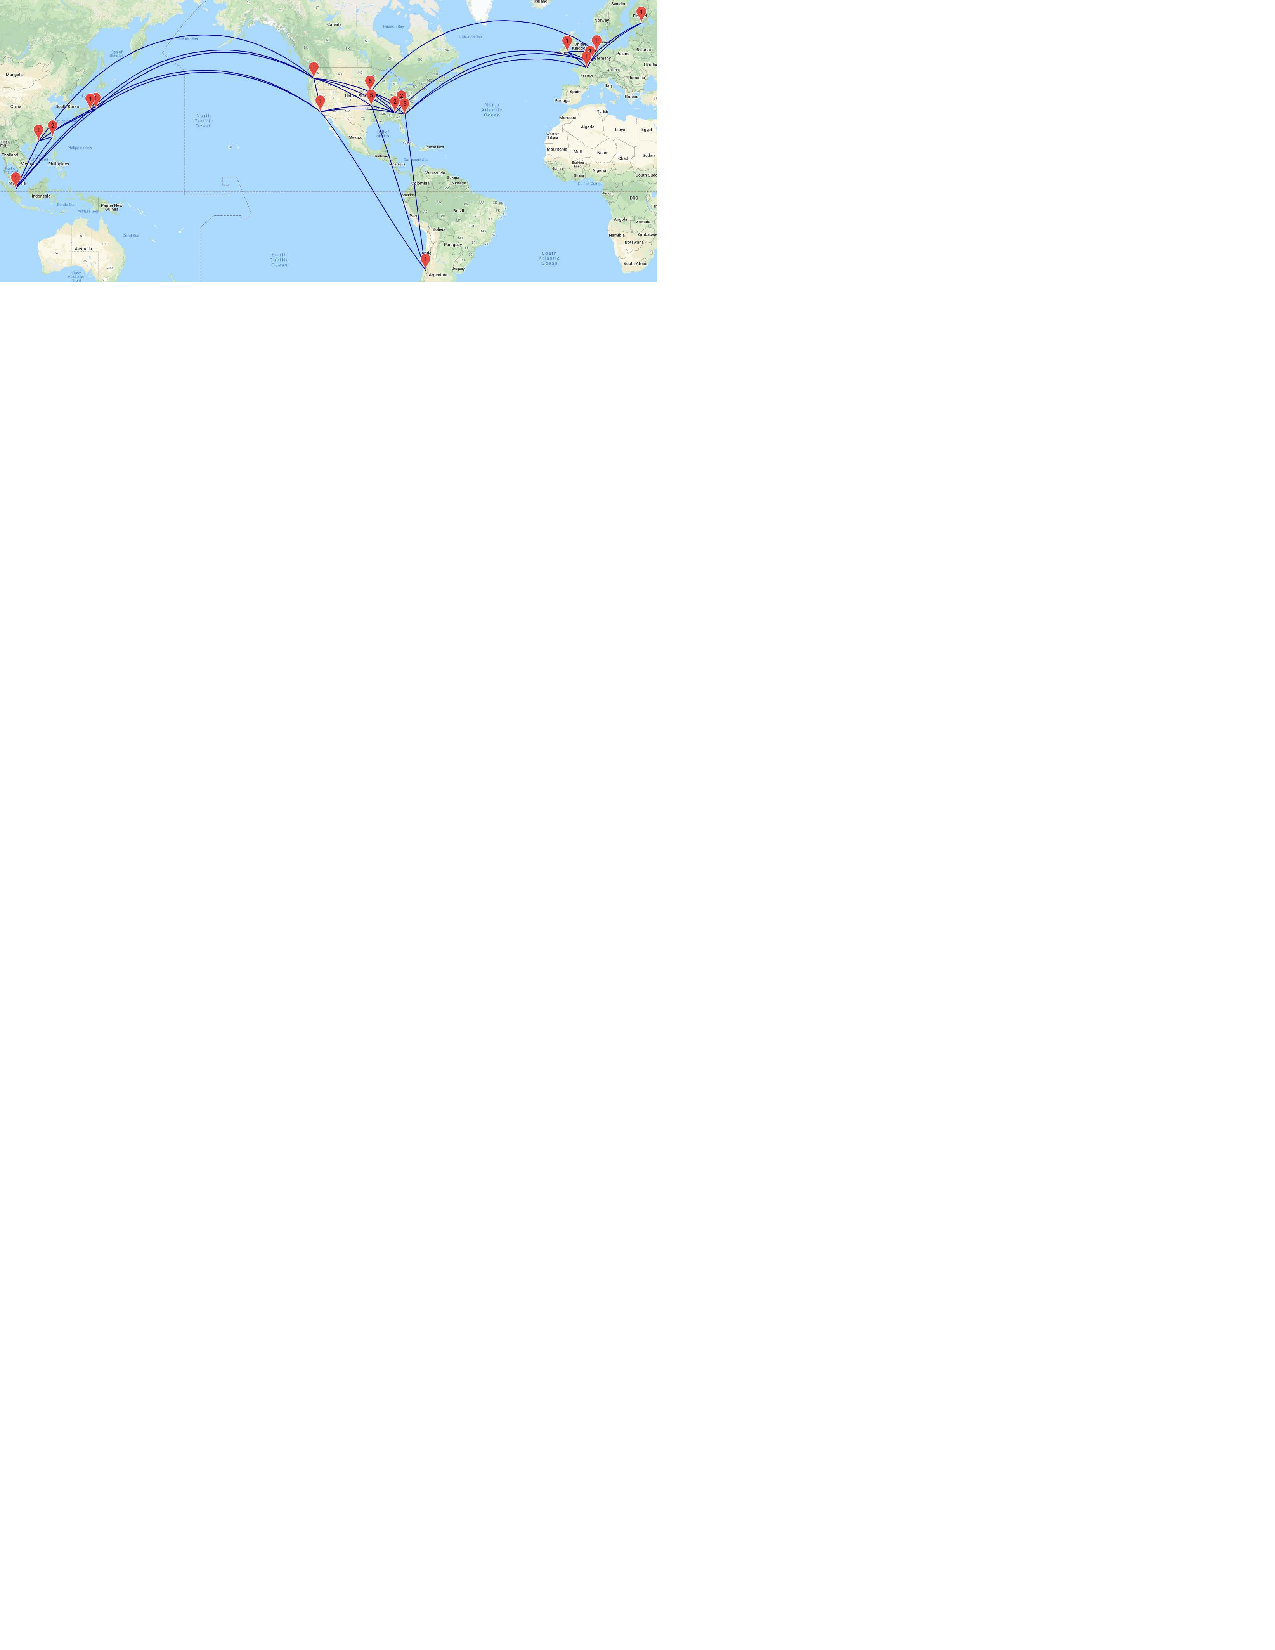
\includegraphics[height=0.6\textheight]{b4.pdf}
        \caption{B4 全球网络}
    \end{figure}
    \only<2>{
        \begin{tikzpicture}[overlay]
            \node [right] at (1cm,4cm) {TE};
            \node [right] at (1cm,3.7cm) {\tiny Traffic};
            \node [right] at (1cm,3.5cm) {\tiny Engineering};
        \end{tikzpicture}
    }
\end{frame}

\begin{frame}
    \frametitle{SLO}
    \framesubtitle{Service Level Objectives 服务级别协议}
    表示 30 天滑动窗口内的网络连接可用性和带宽可用性。
    \begin{table}
        \begin{tabular}{clr}
            \toprule
            服务级别                        & 应用举例           & SLO需求 \\
            \midrule
            \rowcolor<3>{csecondary!30} SC4 & 搜索广告、DNS、WWW & 99.99\% \\
            SC3                             & 照片服务后端、邮件 & 99.95\% \\
            SC2                             & 广告数据库拷贝     & 99.90\% \\
            SC1                             & 搜索索引拷贝       & 99\%    \\
            \rowcolor<2>{ctertiary!30} SC0  & 批量传输           &         \\
            \bottomrule
        \end{tabular}
        \caption{SLO}
    \end{table}
\end{frame}

\section{背景与动机}

%\subsection{扁平架构}
\begin{frame}
    \frametitle{扁平架构}
    \framesubtitle{不利于扩展和可用性}
    之前的 B4 若想增加容量,需要在地理限界内增加站点。但这会带来:
    \begin{enumerate}
        \item 增加了中央流量控制优化算法的运行时间。
        \item 对交换机有限的流表空间增加压力。
        \item 使得容量管理变得复杂并给应用开发者造成麻烦。
    \end{enumerate}
    \only<2>{为了解决这个问题,引入 \emph{supernode}(超级节点)和两层架构。} % 后文讨论细节
\end{frame}

%\subsection{分层架构}
\begin{frame}
    \frametitle{分层架构}
    \framesubtitle{容量不对等问题}
    B4 中 6--20\% 的地理级连接仍然会在 $\geq$ 5\% 的时间内有容量不对等情形。
    \begin{figure}[H]
        \centering
        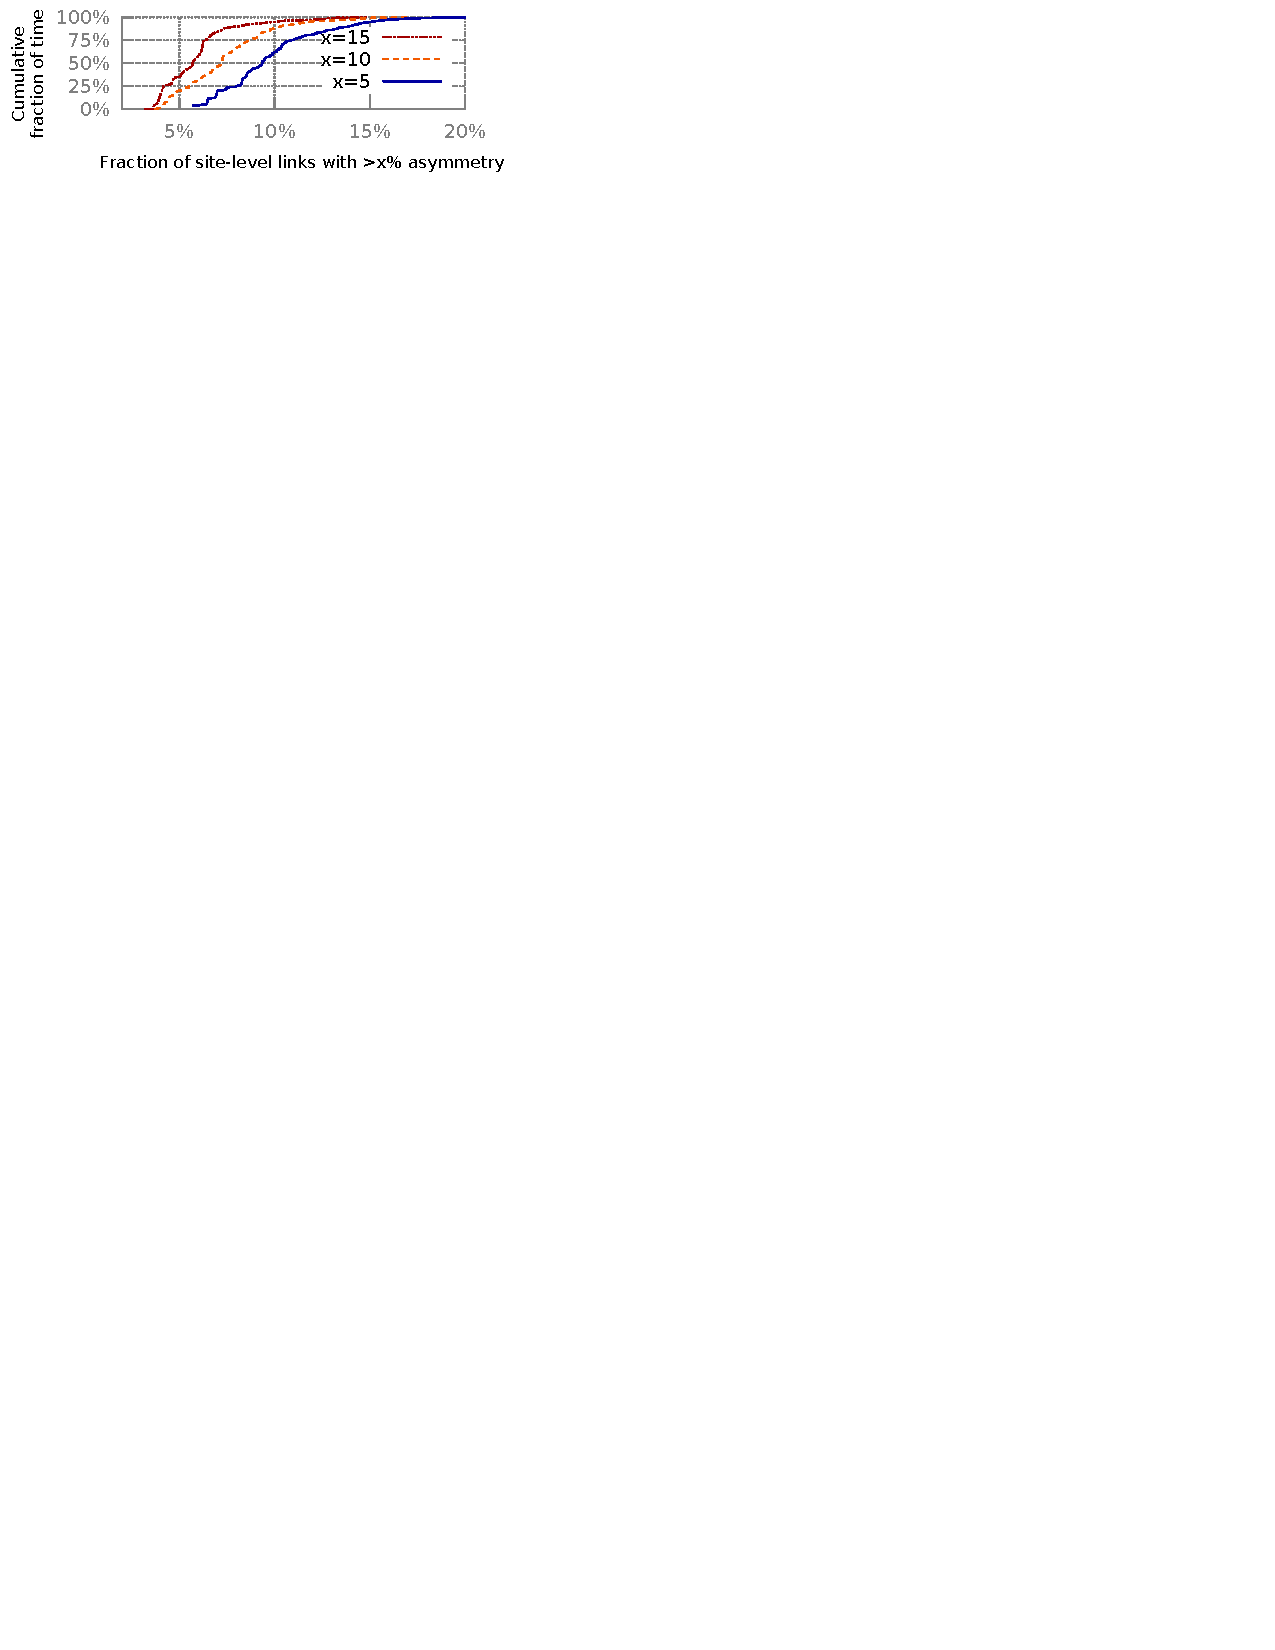
\includegraphics[height=0.5\textheight]{asym}

        $\frac{\text{avg}_{\forall i} C_i - \text{min}_{\forall i} C_i}{\text{avg}_{\forall i} C_i}$
        \caption{地理级容量不对等}\label{fig:asym}
    \end{figure}
\end{frame}

\begin{frame}[label=asym]
    \frametitle{不对等的后果}
    \framesubtitle{大幅减少系统效率}

    \begin{figure}
        \centering
        \begin{tikzpicture}
            \tikzstyle{supernode}=[rectangle,draw,minimum width=1.5cm,minimum height=1cm,fill=white];
            \tikzstyle{flow}=[->];
            \draw[draw=none,fill=cprimary!10]  (-1.5,2) rectangle (0.5,-2);
            \draw[draw=none,fill=cprimary!10]  (1.5,2) rectangle (3.5,-2);
            \node[supernode] (a1) at (-0.5,1) {$A_1$};
            \node [supernode] (b1) at (2.5,1) {$B_1$};
            \node [supernode] (b2) at (2.5,-1) {$B_2$};
            \only<1,3>{
                \node [supernode] (a2) at (-0.5,-1) {$A_2$};
                \draw [flow](-2,-1) node[left]{$\frac{c}{2}$} -- (a2);
            }
            \only<2>{
                \node [supernode,draw=csecondary] (a2) at (-0.5,-1) {\color{csecondary}$A_2$};
                \draw [flow,csecondary](-2,-1) node[left]{\color{csecondary} $\frac{c}{2}$} -- (a2);
            }
            \node at (-0.5,2.5) {Site $A$};
            \node at (2.5,2.5) {Site $B$};
            \draw[flow] (-2,1) node[left] {$\frac{c}{2}$} -- (a1);

            \draw (a1) -- (b2);
            \draw  (a1) edge (b1);
            \only<1>{
                \draw (a2) edge node[above] {5} (b1);
                \draw (a2) edge node[above] {5} (b2);
            }
            \only<2->{
                \draw[csecondary] (a2) edge node[above] {1} (b1);
                \draw[csecondary]  (a2) edge node[above] {1} (b2);
            }
            \draw  (b1) edge node [right] {4} (b2);
            \only<3->{
                \draw[cprimary] (a1) edge node [left] {\emph{sidelink}} node[right] {4} (a2);
            }
        \end{tikzpicture}
        \caption{\only<1>{对等} \only<2->{不对等示例} \only<2>{$c=4$} \only<3>{$c=12$}}\label{fig:asymeg}
    \end{figure}
\end{frame}

\begin{frame}
    \begin{itemize}[<+->]
        \item 使用 \emph{sidelink} 可以提高不对等时的带宽利用率。但是仍然需要考虑相关的协议问题,比如有些数据不可分割、MAC 地址不可变化,后文通过基于划分的哈希解决(算法 \ref{alg:hash})。
        \item 以及死循环问题,转换隧道可能是\emph{原子操作},以任意顺序应用 TE 更新会导致这种死循环率上升,后文通过TSG排序算法解决(算法 \ref{alg:tsgseq})。
        \item Merchant 交换机只支持有限的匹配和哈希规则,通过双层匹配(算法 \ref{alg:fgmatch})和基于划分的哈希(算法 \ref{alg:hash})减少流表规则数量上的压力。
    \end{itemize}
\end{frame}

\section{站点拓扑的进化}

\begin{frame}
    \frametitle{Saturn}
    \framesubtitle{第一代 B4 网络结构}
    \begin{columns}
        \begin{column}{0.4\textwidth}
            \begin{figure}
                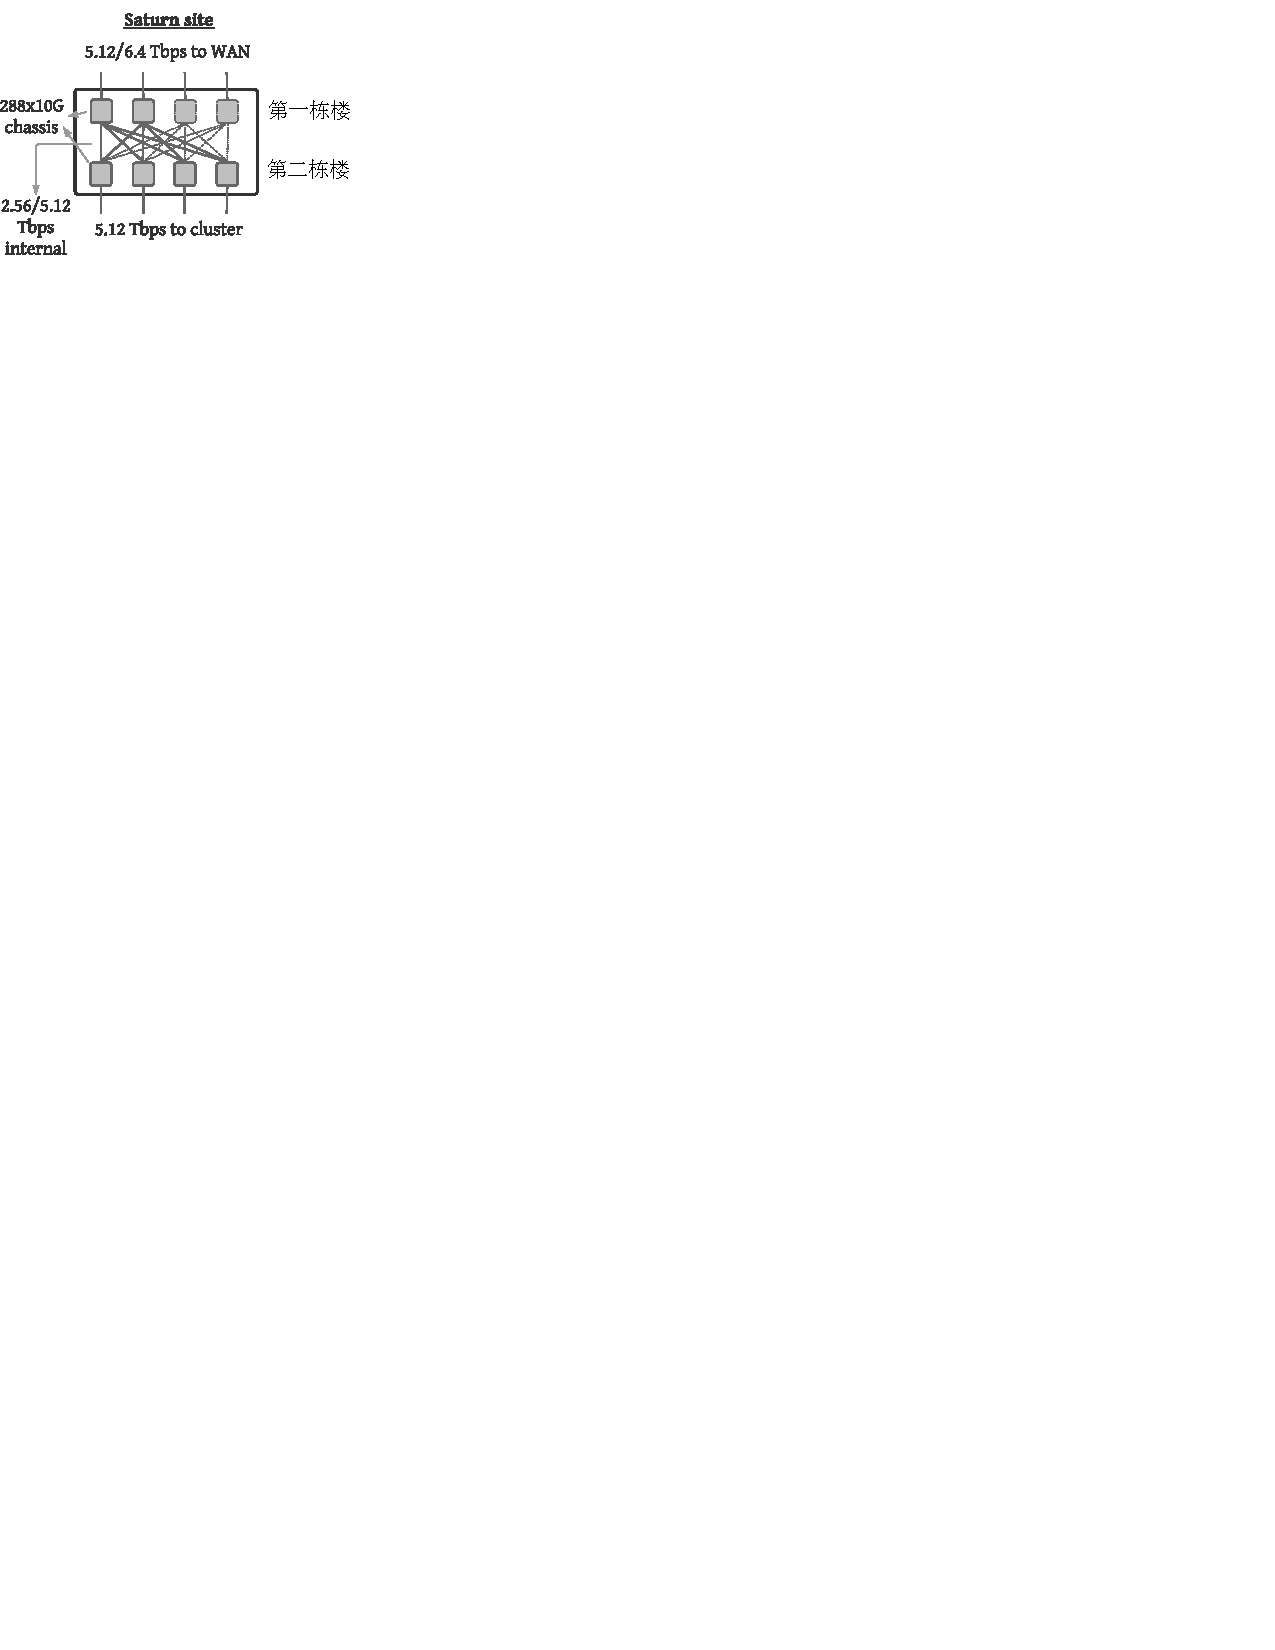
\includegraphics[width=\linewidth]{saturn}
                \caption{Saturn 站点}
            \end{figure}
        \end{column}
        \begin{column}{0.6\textwidth}
            \begin{table}
                \begin{tabular}{>{\bfseries}ll}
                    \toprule
                    名称             & Saturn                               \\
                    部署年           & 2010                                 \\
                    类型             & 数据中心                             \\
                    交换机芯片       & 24x10G                               \\
                    每站点机箱数     & 6 / 8                                \\
                    站点容量 (Tbps)  & 5.12 \textsc{ex} 2.56 \textsc{inter} \\
                    每站点交换机箱数 & 4                                    \\
                    控制域数量       & 1                                    \\
                    \bottomrule
                \end{tabular}
                \caption{Saturn 站点}\label{tab:saturn}
            \end{table}
        \end{column}
    \end{columns}
\end{frame}

\begin{frame}
    \frametitle{Jumpgate: JPOP}
    \framesubtitle{仅传输站点}
    \begin{columns}
        \begin{column}{0.4\textwidth}
            \begin{figure}
                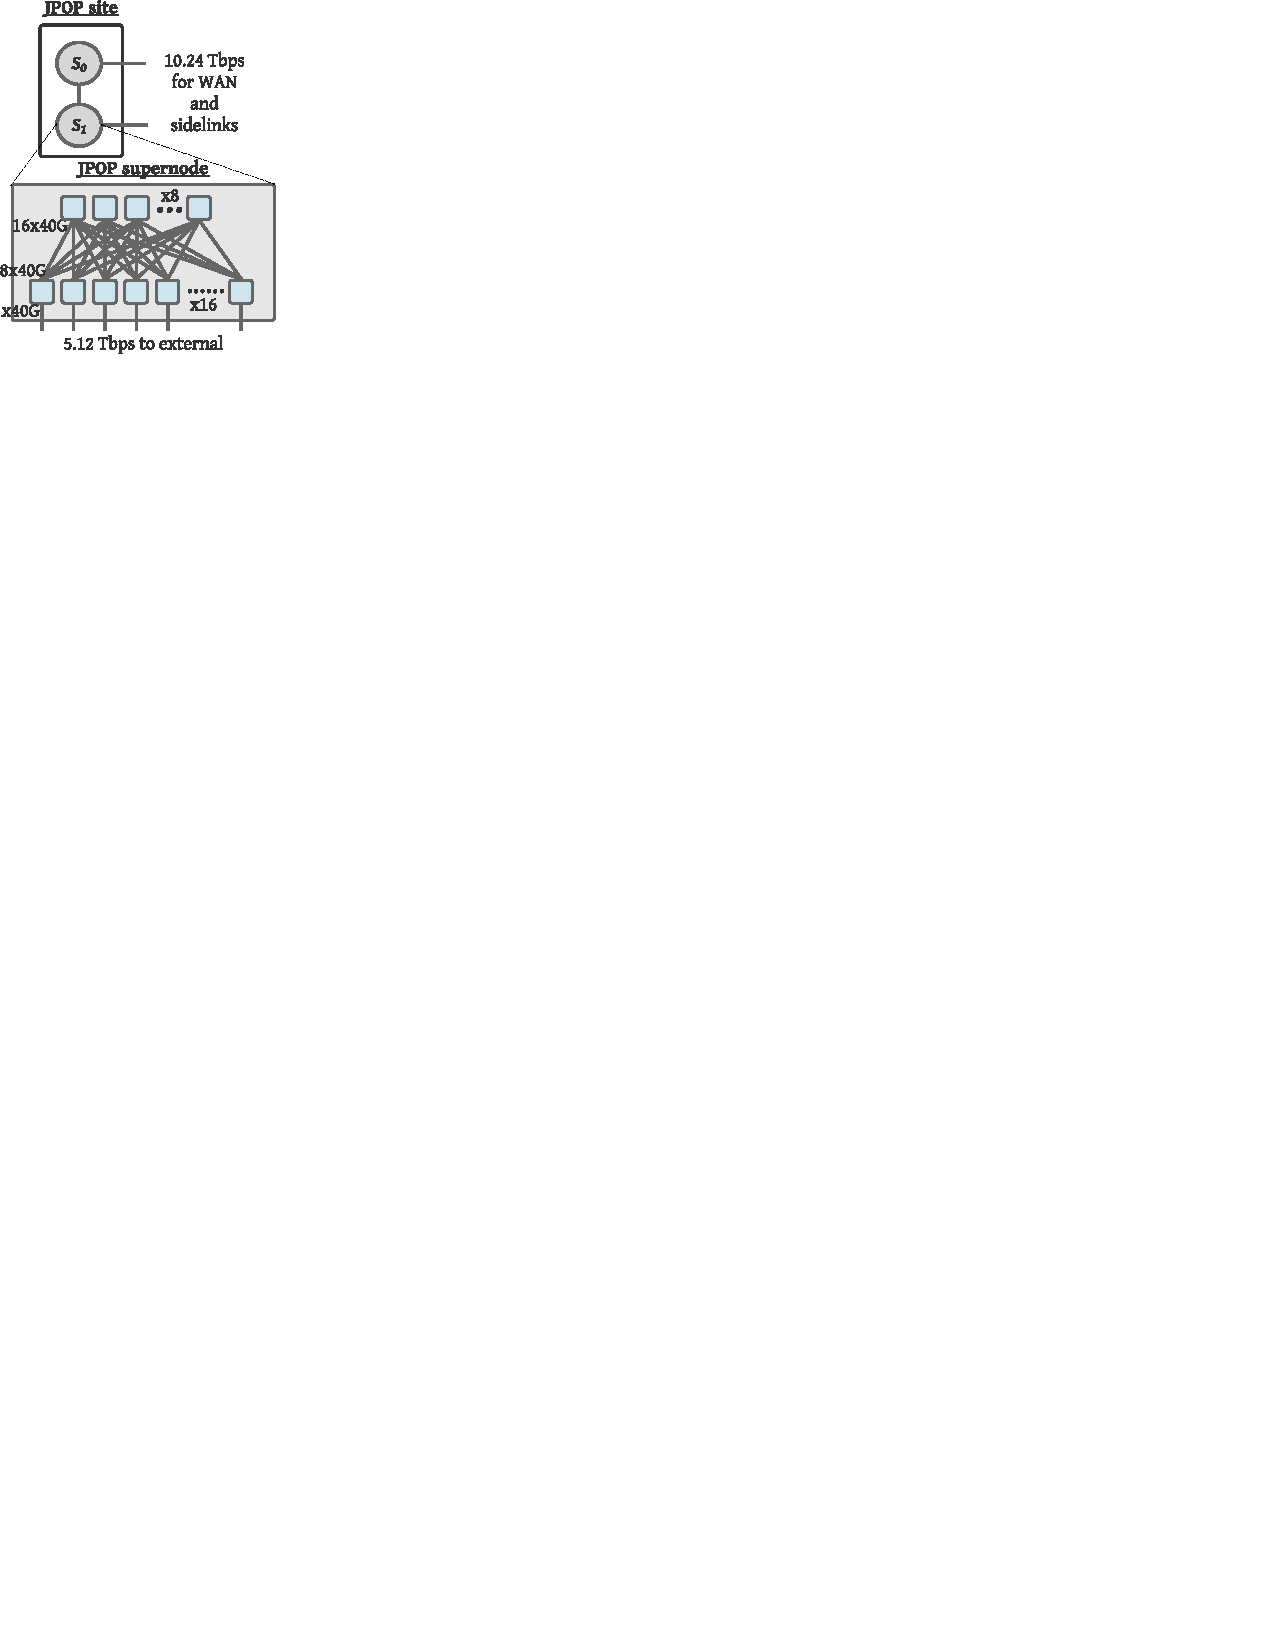
\includegraphics[height=0.7\textheight]{jpop}
                \caption{JPOP 站点}
            \end{figure}
        \end{column}
        \begin{column}{0.6\textwidth}
            \begin{table}
                \begin{tabular}{>{\bfseries}ll}
                    \toprule
                    名称             & JPOP   \\
                    部署年           & 2013   \\
                    类型             & \color{cprimary} POP    \\
                    交换机芯片       & 16x40G \\
                    每站点机箱数     & 20     \\
                    \color{cprimary} 超级节点交换机数 & 24     \\
                    站点容量 (Tbps)  & 10.24  \\
                    每站点交换机箱数 & 4      \\
                    控制域数量       & 2      \\
                    \bottomrule
                \end{tabular}
                \caption{JPOP 站点}\label{tab:jpop}
            \end{table}
        \end{column}
    \end{columns}
\end{frame}

\begin{frame}
    \frametitle{Jumpgate: Stargate}
    \framesubtitle{数据中心级}
    \begin{columns}
        \begin{column}{0.4\textwidth}
            \begin{figure}
                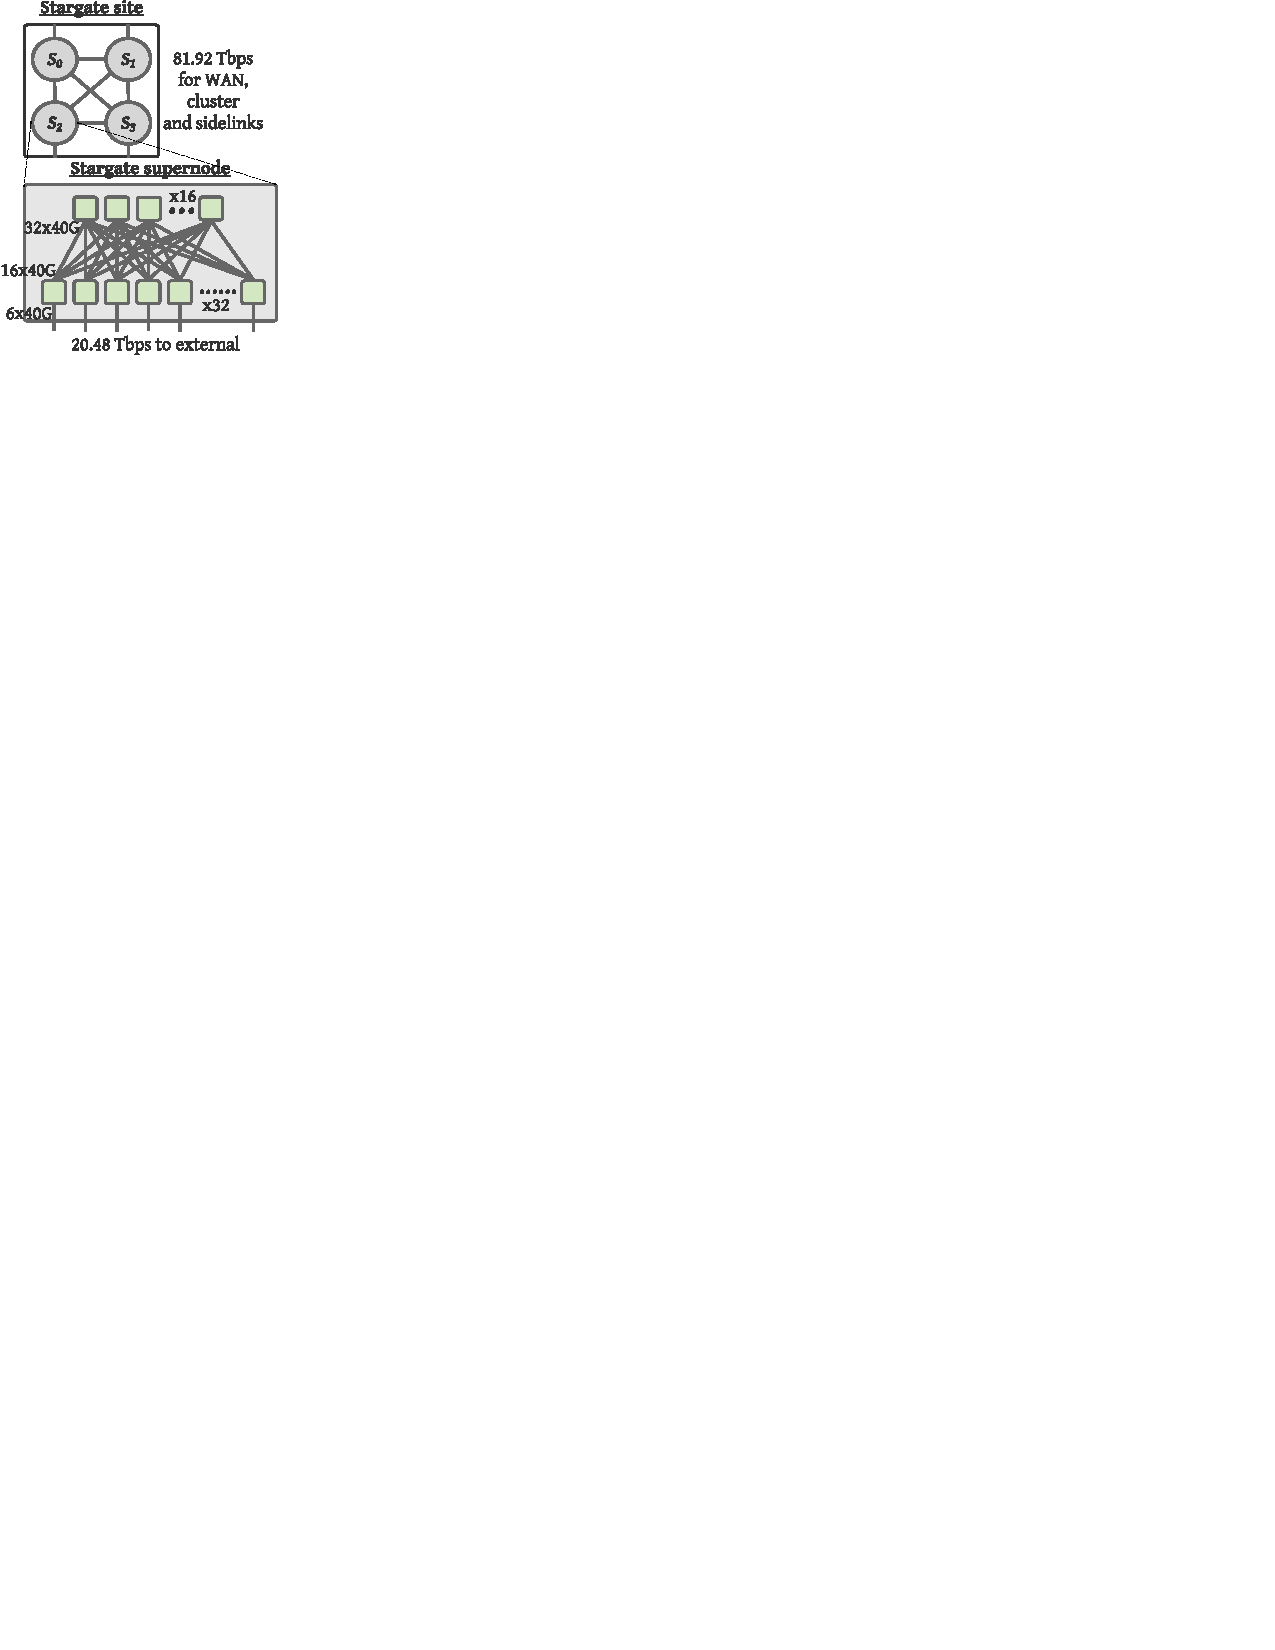
\includegraphics[height=0.7\textheight]{stargate}
                \caption{Stargate 站点}
            \end{figure}
        \end{column}
        \begin{column}{0.6\textwidth}
            \begin{table}
                \begin{tabular}{>{\bfseries}ll}
                    \toprule
                    名称             & Stargate \\
                    部署年           & 2014     \\
                    类型             & 数据中心 \\
                    交换机芯片       & 32x40G   \\
                    每站点机箱数     & 192      \\
                    超级节点交换机数 & 48       \\
                    站点容量 (Tbps)  & 81.92    \\
                    每站点交换机箱数 & 8        \\
                    控制域数量       & 4        \\
                    \bottomrule
                \end{tabular}
                \caption{Stargate 站点}\label{tab:stargate}
            \end{table}
        \end{column}
    \end{columns}
\end{frame}

\begin{frame}
    \frametitle{Jumpgate: Stargate}
    \framesubtitle{带来的好处}

    \begin{columns}
        \begin{column}{0.2\textwidth}
            \begin{figure}
                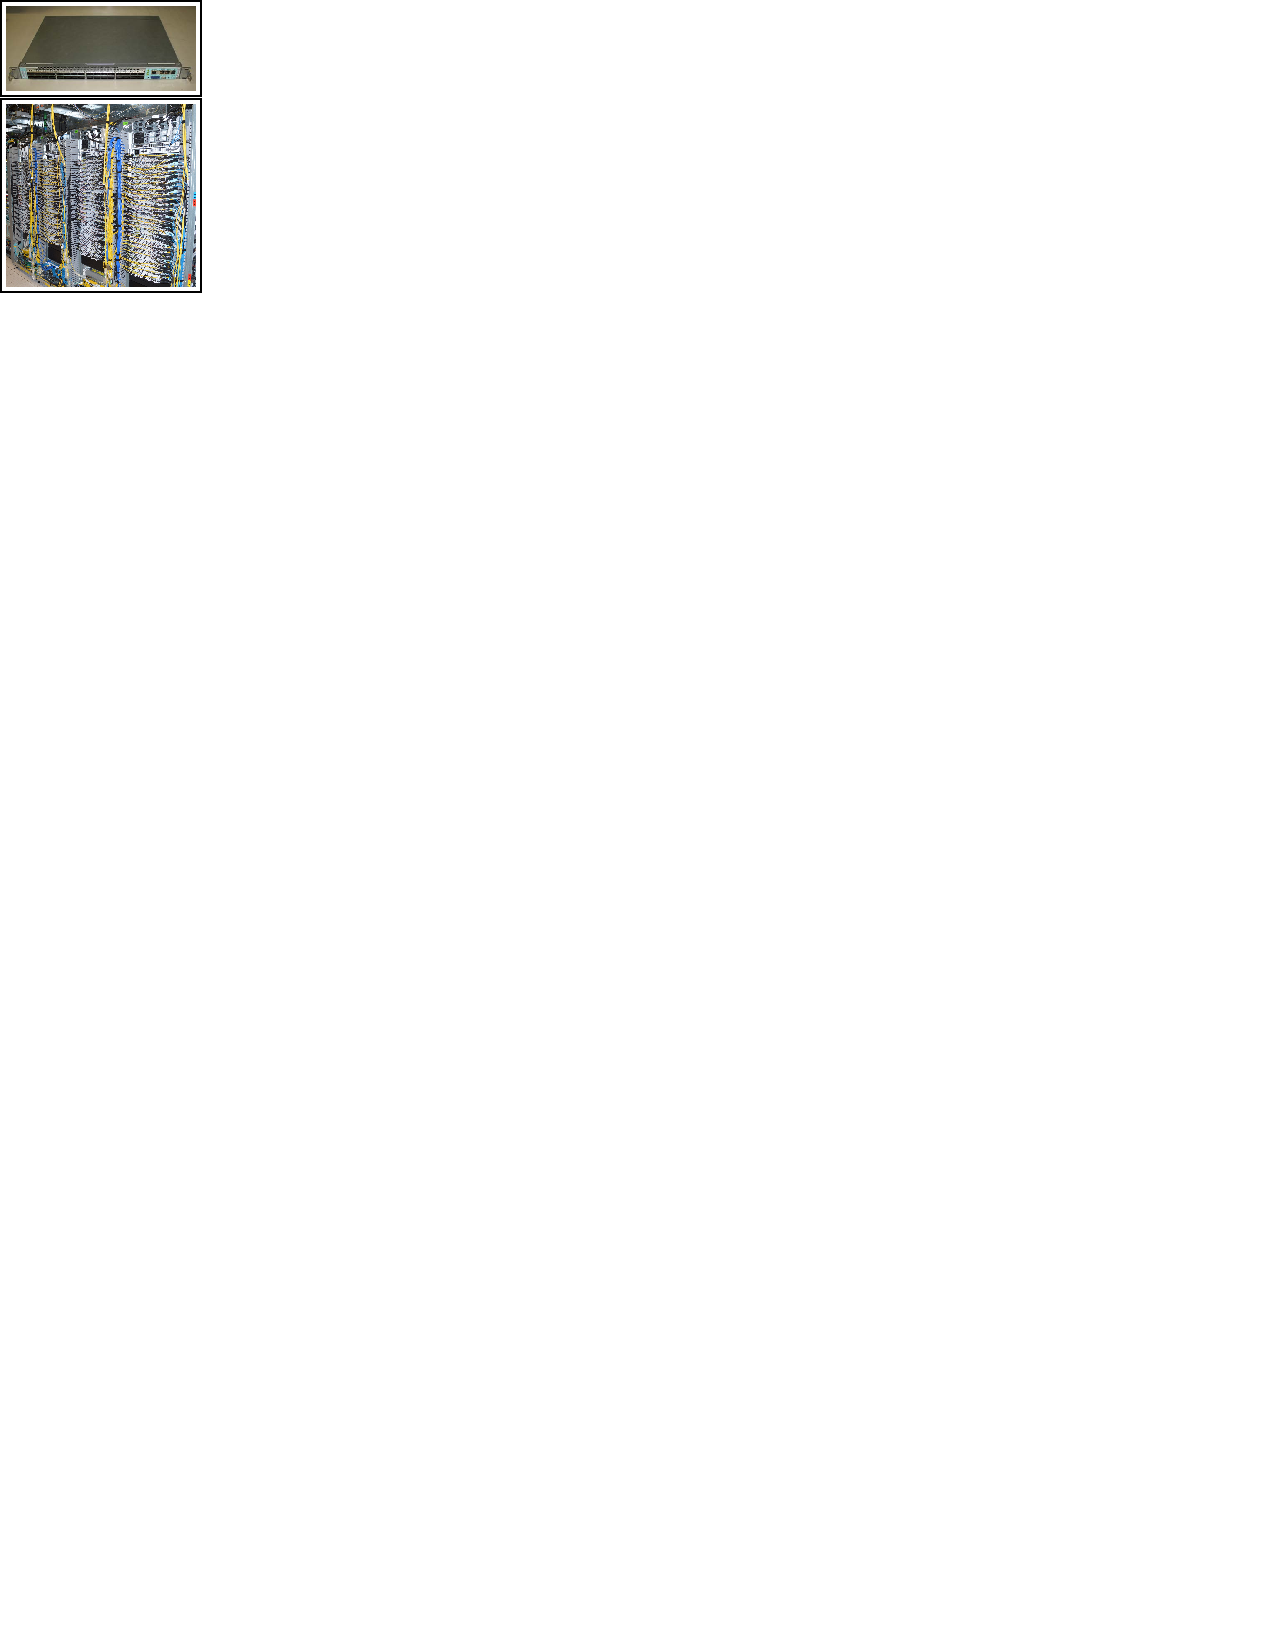
\includegraphics[width=\linewidth]{stargateswitch}
                \caption{交换机与交换机架}
            \end{figure}
        \end{column}
        \begin{column}{0.6\textwidth}
            这种模型简化了网络建模、容量规划和管理。
            \begin{figure}
                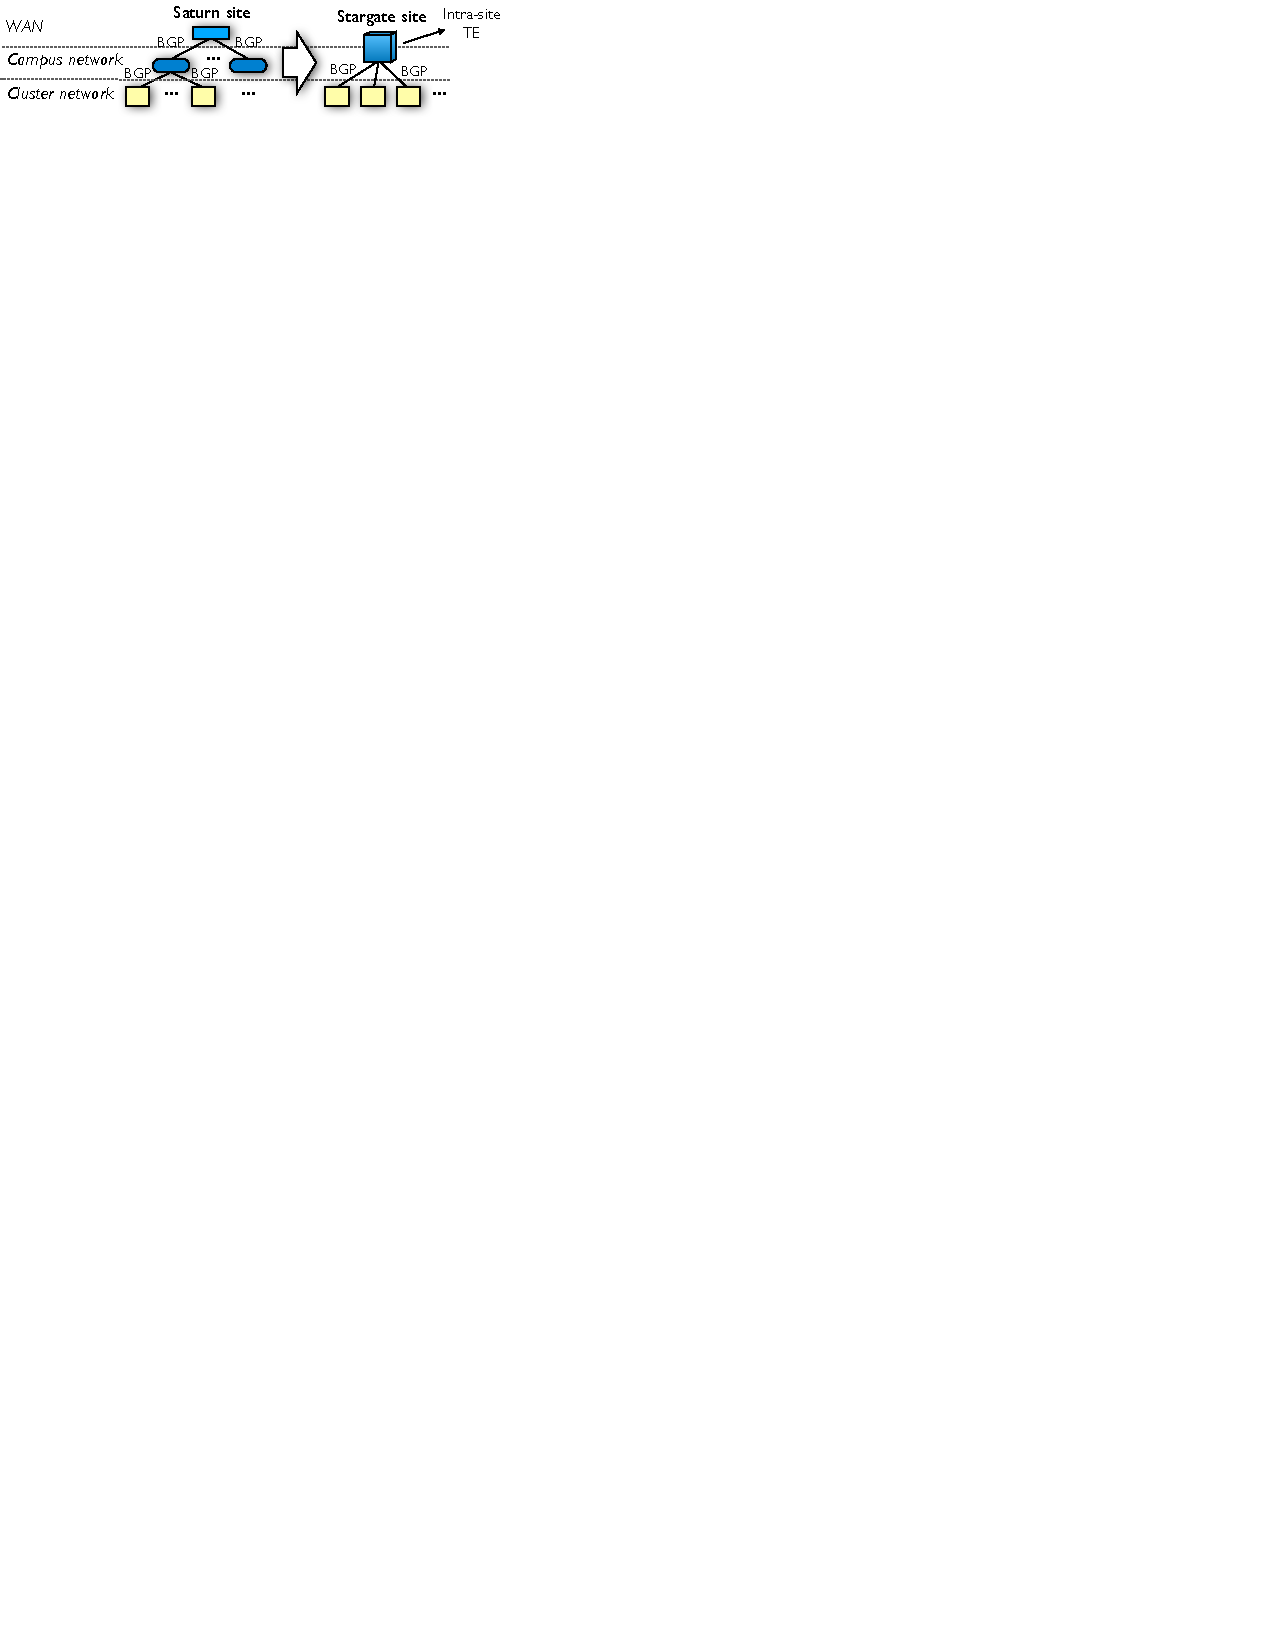
\includegraphics[width=\linewidth]{stargatesubsumes}
                \caption{减少 BGP 复杂度}
            \end{figure}
        \end{column}
    \end{columns}
\end{frame}

\begin{frame}[plain]
    \frametitle{Facebook Outage}
    \framesubtitle{BGP 相关新闻}
    Facebook 在 10 月 4 日爆发了服务大中断,其他网络无法与之形成正确的连接。
    \begin{figure}
        \centering
        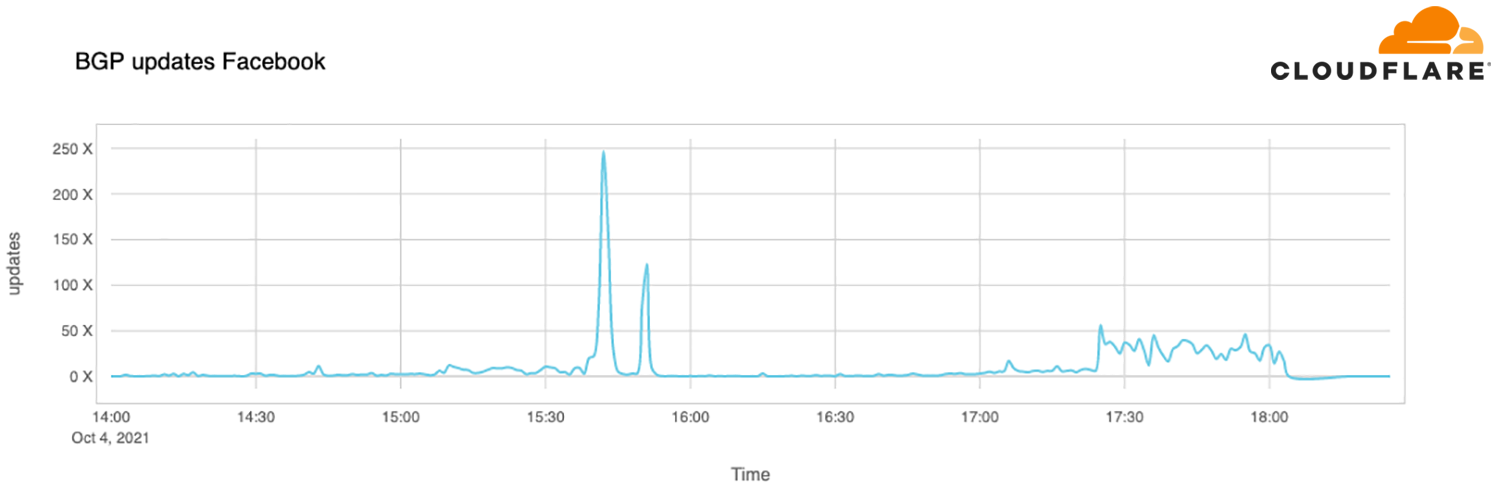
\includegraphics[width=\linewidth]{bgp}
        \caption{BGP 变更高峰\footfullcite{cloudflarebgp}}
    \end{figure}
\end{frame}

\section{分层流量工程}

%\subsection{简单粗暴的提案}
\begin{frame}
    \frametitle{简单粗暴的提案}
    \framesubtitle{平面流量工程}
    \highlight[csecondary]{方法:集中式路由选择算法}~直接对站点内所有的超级节点直接应用流量控制。这种模型下,由一个中央控制器使用 IP-in-IP 封装对超级节点级隧道进行负载均衡。

    \paragraph{缺点} 高运行时间、花费大量的交换机流表空间、不可扩展。每个站点内有4个超级节点,那么站点到站点间的3跳转发会有$4^3=64$条路径。
\end{frame}

\begin{frame}
    \frametitle{简单粗暴的提案}
    \framesubtitle{最短路转发}

    \highlight[csecondary]{方法:分散式路由选择算法}~超级节点级链路实现最短路转发。

    \paragraph{优点}拥有扩展性、只需要一层封装、在广域网失效时能够通过\alert{旁路链接}完成流量转移。

    \paragraph{缺点}无法处理容量不对等情形,不是完全失效的情况下无法找到通过\alert{旁路链接}得到的更长但容量更大的路径。
    \hyperlink{asym<3>}{\beamergotobutton{不对等的后果}}
\end{frame}

%\subsection{分层流量工程结构}
\begin{frame}
    \frametitle{分层流量工程结构}
    \framesubtitle{概念}
    \begin{columns}
        \begin{column}{0.6\textwidth}
            \begin{itemize}
                \item[SSG] \emph{Switch Split Group} 确定物理交换机所分割的流量。
                \item[TSG] \emph{Tunnel Split Group} 确定一个链路\emph{tunnel}内如何分配两个站点超级节点间的流量分布。
                \item[TG] \emph{Tunnel Group} 通过 IP-in-IP 封装映射 FG 到一个链路集合。
                \item[FG] \emph{Flow Group} $\langle$源站点, 目标站点, 服务类别$\rangle$
            \end{itemize}
        \end{column}
        \begin{column}{0.4\textwidth}
            \begin{figure}
                \centering
                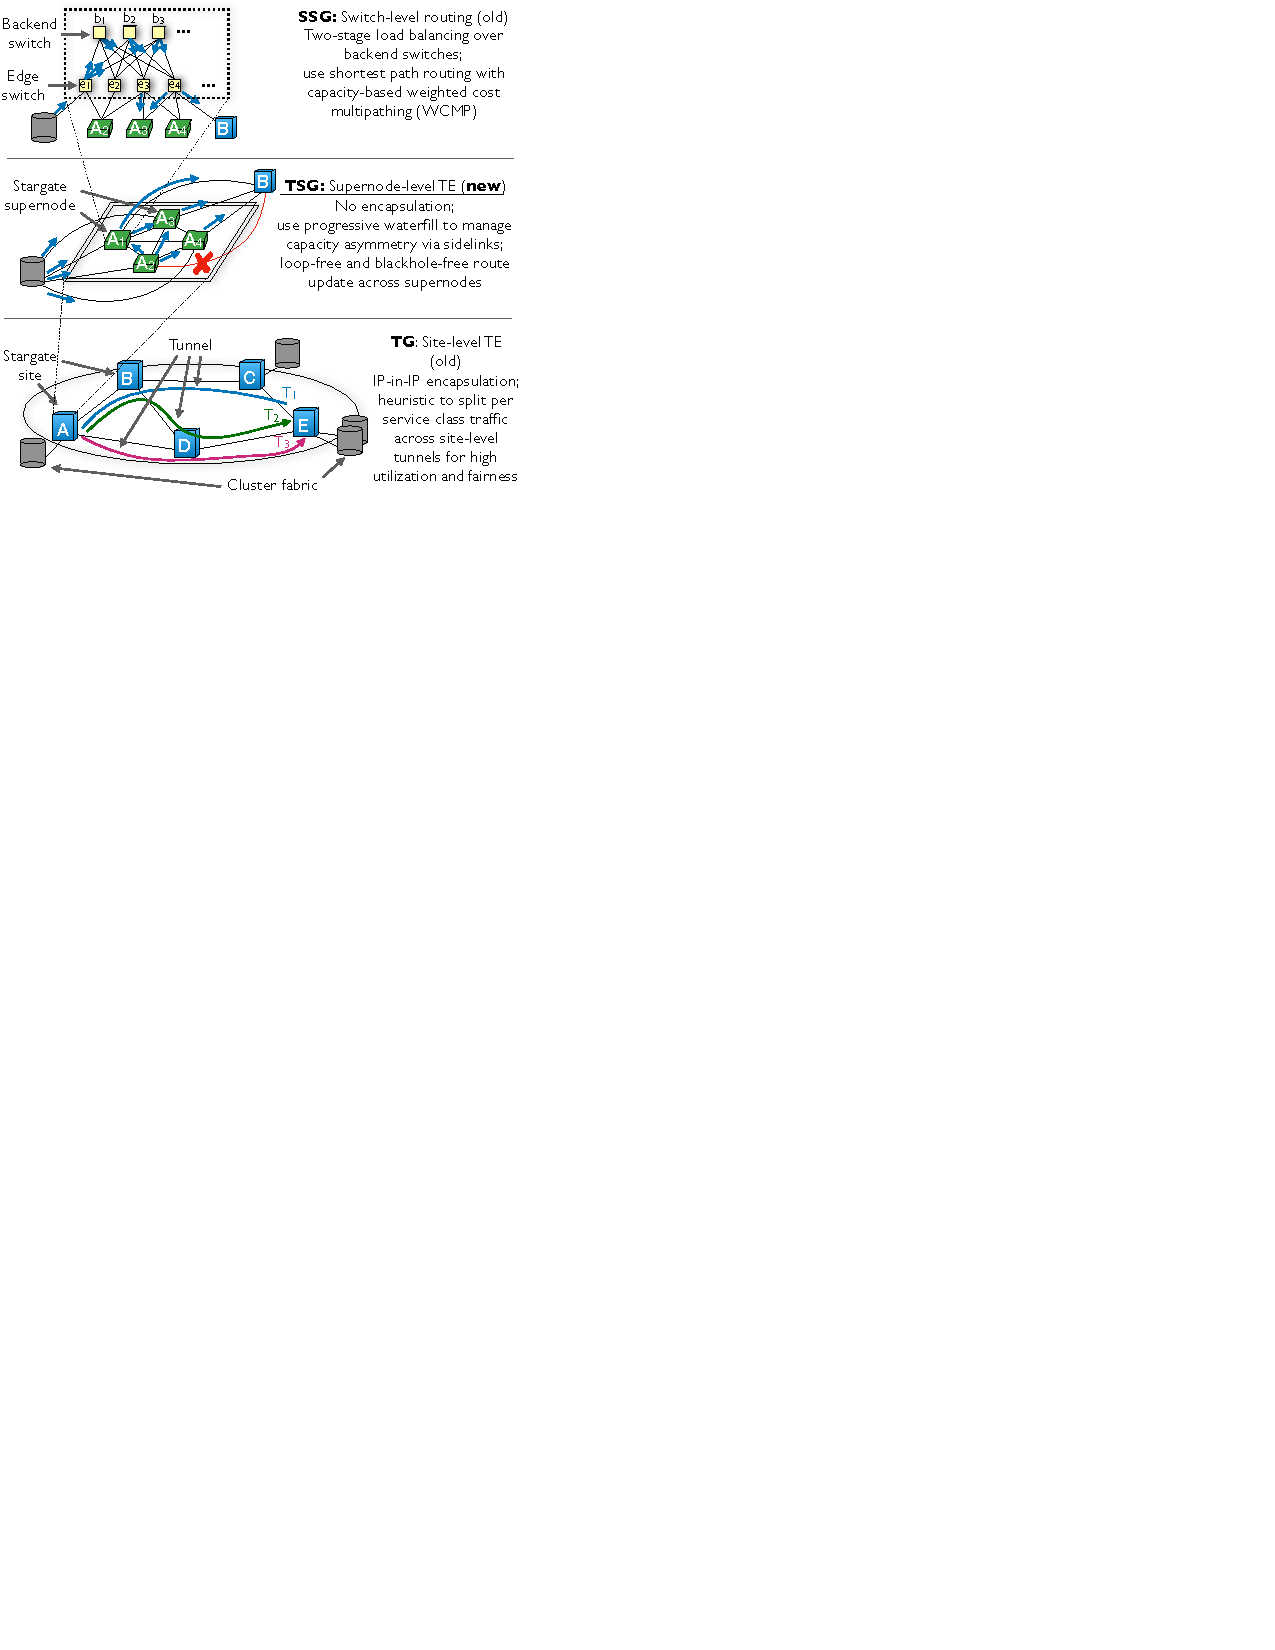
\includegraphics[width=0.9\linewidth]{hitearch}
                \caption{不同的流量工程结构}
            \end{figure}
        \end{column}
    \end{columns}
\end{frame}

\begin{frame}
    \frametitle{分层流量工程结构}
    \framesubtitle{运行概览}
    \begin{columns}
        \begin{column}{0.6\textwidth}
        \begin{algorithm}[H]
            \caption{B4 运行概览}
            域控制器通过聚合可用的物理链路容量来计算超级节点间的连接\;
            中央控制器根据上述结果计算 TSG 来分配每一条站点级的出口连接\;
            \leIf{对等}{不使用旁路连接\;}{通过旁路连接重新分配TSG}
            使用上述 TSG 结果计算站点级每条链路的有效容量,生成 TG\;
            生成 TE 操作的无环依赖图\;
            通过生成 SSG 分割规则,按照次序对 FG, TG, TSG 编程\;
        \end{algorithm}
        \end{column}
        \begin{column}{0.4\textwidth}
            \begin{figure}
                \centering
                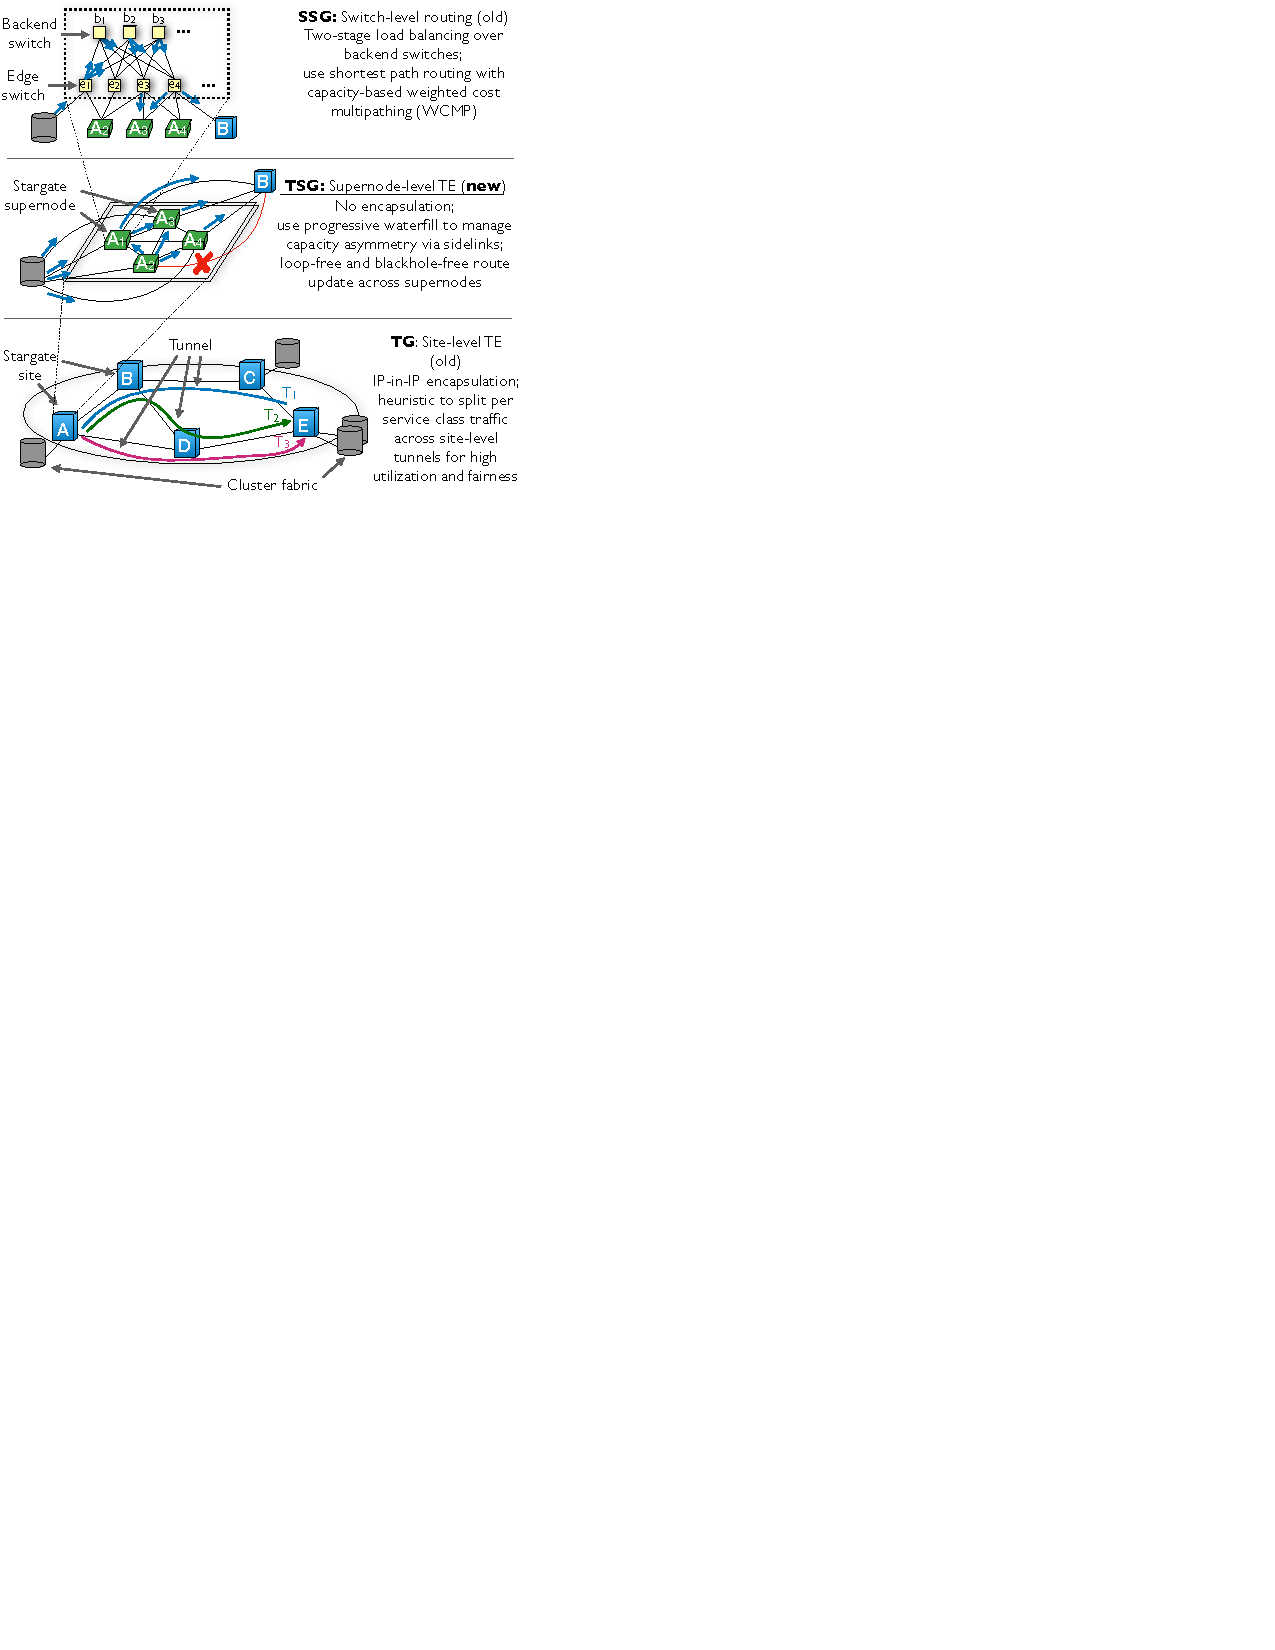
\includegraphics[width=0.9\linewidth]{hitearch}
            \end{figure}
        \end{column}
    \end{columns}
\end{frame}

%\subsection{TSG生成算法}
\begin{frame}
    \frametitle{TSG 生成算法}
    \framesubtitle{问题描述}
    假设进入隧道的流量对于源站点的所有超级节点来说都是平均分割的。对于沿着隧道的每个站点内的每一个超级节点计算 TSG,使得能够最大化利用对应超级节点连接容量的上限。使用正整数表示输出链路上的每一连接的相对权重,并要求每一个 TSG 的权重总和不能超过一个阈值 $T$,因为交换器哈希表键值数量限制。
    
    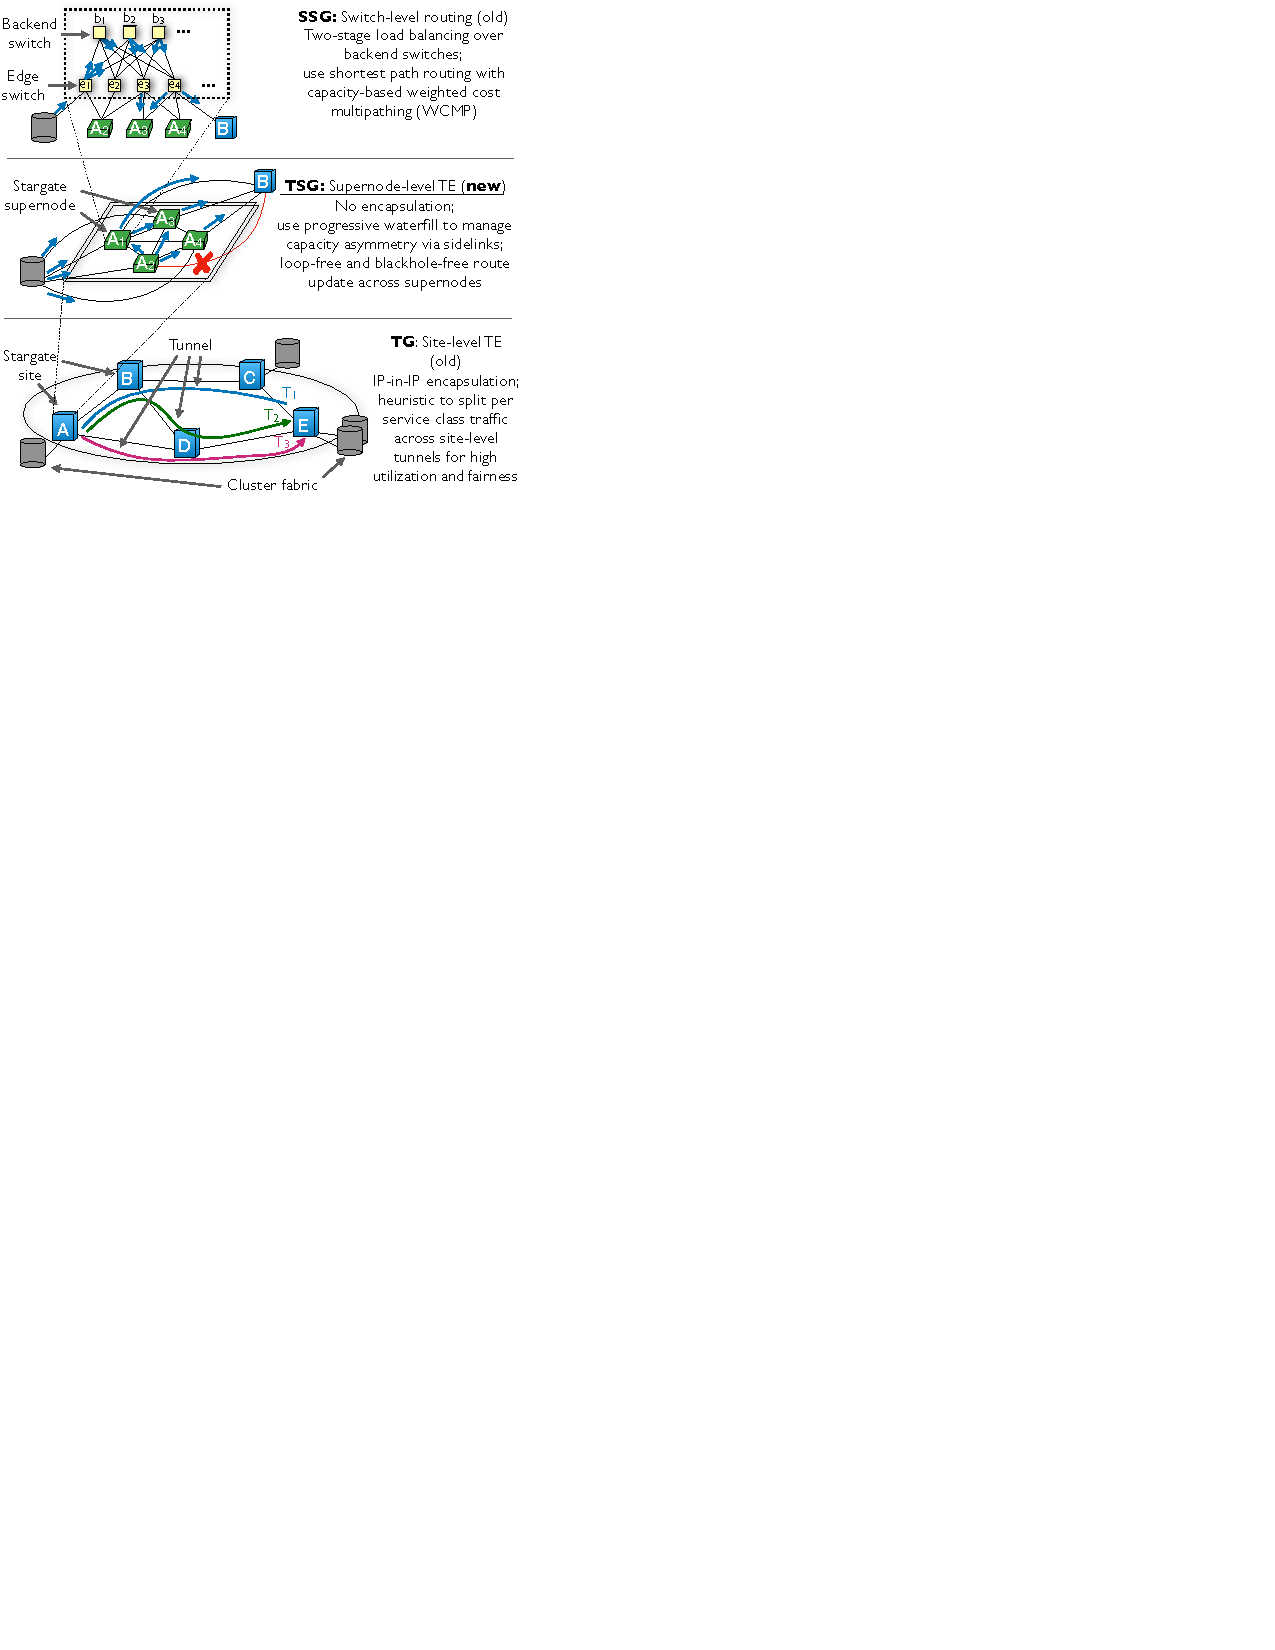
\includegraphics[trim={0 6cm 0 11cm},clip]{hitearch}
\end{frame}

\begin{frame}
    \frametitle{TSG 生成算法}
    \framesubtitle{例子\only<4->{(罕见)}}
    \begin{figure}
        \centering
        \begin{tikzpicture}
            \tikzstyle{supernode}=[rectangle,draw,minimum width=1cm,minimum height=0.7cm,fill=white];
            \tikzstyle{flow}=[->, line width=1pt];
            \node [supernode] (a1) at (-1.5,1.5) {$A_1$};
            \node [supernode] (a2) at (-1.5,-0.5) {$A_2$};
            \node [supernode] (b1) at (1,1.5) {$B_1$};
            \node [supernode] (b2) at (1,-0.5) {$B_2$};
            \node [supernode] (c1) at (3.5,1.5) {$C_1$};
            \node [supernode] (c2) at (3.5,-0.5) {$C_2$};
            \only<1-4>{
                \draw  (a1) edge (a2);
            }
            \only<5,6>{
                \draw [flow] (a2) edge node [right] {\only<5>{$3c/8$}\only<6>{$c/2$}} (a1);
            }
            \draw  (c1) edge (c2);
            \path [flow] (-3,1.5) edge node[above] {\only<1>{$2c$}\only<2,4>{$c$}\only<3>{$1.5c$}\only<5>{$9c/8$}} (a1);
            \path [flow] (-3,-0.5)  edge node[above] {\only<1>{$2c$}\only<2,4>{$c$}\only<3>{$1.5c$}\only<5>{$9c/8$}} (a2);
            \only<1-3,5,6>{
                \draw [flow] (a1) edge node [above,sloped] {\only<1,6>{$c$}\only<2>{$0.5c$}\only<3>{$0.75c$}\only<5>{$6c/8$}} (b1);
                \draw [flow] (a2) edge node [above,sloped] {\only<1,6>{$c$}\only<2>{$0.5c$}\only<3>{$0.75c$}\only<5>{$6c/8$}} (b1);
            }
            \only<4>{
                \draw (a1) edge (b1);
                \draw (a2) edge (b1);
            }
            \draw [flow] (a1) edge node [above,sloped] {\only<1,4,6>{$c$}\only<2>{$0.5c$}\only<3>{$0.75c$}\only<5>{$6c/8$}} (b2);
            \only<1-4>{
                \draw [flow] (a2) edge node [above,sloped] {\only<1,4>{$c$}\only<2>{$0.5c$}\only<3>{$0.75c$}} (b2);
            }
            \only<5,6>{
                \draw [dashed] (a2) edge (b2);
            }
            \only<1>{
                \draw [flow] (b1) edge node [above,sloped] {$c$} (c1);
                \draw [flow] (b1) edge node [above,sloped] {$c$} (c2);
                \draw  (b2) edge (b1);
            }
            \only<2>{
                \draw [dashed] (b1) edge (c1);
                \draw [dashed] (b1) edge (c2);
                \draw [flow] (b1) edge node [right] {$c$} (b2);
            }
            \only<3,5,6>{
                \draw [dashed] (b1) edge (c1);
                \draw [flow] (b1) edge node [above,sloped] {$c$} (c2);
                \draw [flow] (b1) edge node [right] {\only<3>{$0.5c$}\only<5>{$4c/8$}\only<6>{$c$}} (b2);
            }
            \only<4>{
                \draw [dashed] (b1) edge (c1);
                \draw [dashed] (b1) edge (c2);
                \draw [dashed] (b1) edge (b2);
            }
            \draw [flow] (b2) edge node [above,sloped] {\only<1-4,6>{$c$}\only<5>{$5c/8$}} (c1);
            \draw [flow] (b2) edge node [above,sloped] {\only<1-4,6>{$c$}\only<5>{$5c/8$}} (c2);
            \path [flow] (c1)  edge node[above] {\only<1>{$2c$}\only<2,4>{$c$}\only<3>{$c$}\only<5>{$5c/8$}\only<6>{$c$}}  (5,1.5);
            \path [flow] (c2)  edge node[above] {\only<1>{$2c$}\only<2,4>{$c$}\only<3>{$2c$}\only<5>{$13c/8$}\only<6>{$2c$}}  (5,-0.5);
        \end{tikzpicture}
        \caption{
            \only<1>{对等网络 $TC=4c$}
            \only<2>{不对等网络 $TC=2c$}
            \only<3>{不对等网络 $TC=3c$}
            \only<4>{$TC=0$ ($B_1$故障)\footnote{\hyperlink{notclose}{\beamergotobutton{不关闭的后果}}} 或 $TC=2c$ ($B_1$关闭)}
            \only<5>{$TC=9c/4$ (次优解)}
            \only<6>{$TC=3c$ (最优解)}
        }
    \end{figure}
\end{frame}

\begin{frame}[plain,label=notclose]
    \frametitle{不关闭的后果}
    最近的一次 lab 含有环路的网络,代码写的不好的话,如果切断一个链路,而没有告知另一侧的路由,将会导致另一侧的路由仍然会向错误的链路发包,导致不可达。

    \begin{figure}
        \begin{tikzpicture}
            \tikzstyle{host}=[draw]
            \tikzstyle{switch}=[draw]
            \tikzstyle{connection}=[]
            \tikzstyle{constr}=[right,font=\ttfamily\small]
            \node (h1) [host] at (-0.5,0.5) {h1};
            \node (s1) [switch] at (1.5,0.5) {s1};
            \only<1,2>{
                \node (s3) [switch] at (3,2) {s3};
            }
            \only<3>{
                \node (s3) [switch,opacity=0.5] at (3,2) {s3};
            }
            \node (s2) [switch] at (4.5,0.5) {s2};
            \node (s4) [switch] at (3,-1) {s4};
            \node (h2) [host] at (6.5,0.5) {h2};
            \draw[line width=1pt] (h1) edge (s1);
            \only<1>{
                \draw[line width=1pt] (s1) edge (s3);
            }
            \only<1>{
                \draw (s1) edge (s4);
            }
            \only<2->{
                \draw[line width=1pt] (s1) edge (s4);
            }
            \only<1>{
                \draw[line width=1pt] (s3) edge (s2);
            }
            \only<2>{
                \draw[line width=1pt,->,csecondary] (s2) edge (s3);
            }
            \only<1>{
                \draw (s4) edge (s2);
            }
            \only<2>{
                \draw[line width=1pt,->] (s4) edge (s2);
            }
            \only<3>{
                \draw[line width=1pt] (s4) edge (s2);
            }
            \draw[line width=1pt] (s2) edge (h2);
        \end{tikzpicture}
        \caption{\only<1>{正常链路}
            \only<2>{不可达}
            \only<3>{关闭后}}
    \end{figure}
\end{frame}

\begin{frame}[plain]
    \frametitle{网络流算法}
    \framesubtitle{回顾}
    \begin{columns}
        \begin{column}{0.5\textwidth}
            \begin{algorithm}[H]
                \caption{Augment($f,c,P$)}
                $\delta\Leftarrow$ bottleneck capacity of augmenting path $P$\;
                \ForEach(){$e\in P$}{
                    \If(){$e\in E$}{
                        $f(e)\leftarrow f(e)+\delta$\;
                    }
                    \Else(){
                        $f(e^R)\leftarrow f(e^R)-\delta$\;
                    }
                }
                \Return{$f$}\;
            \end{algorithm}
        \end{column}
        \begin{column}{0.5\textwidth}
            \begin{algorithm}[H]
                \caption{Ford-Fulkerson Algorithm}
                \KwIn{$G=(V,E),c,s,t$}
                \ForEach(){$e\in E$}{
                    $f(e)\leftarrow 0$\;
                }
                $G_f\leftarrow$ residual graph\;
                \While(){there exists augmenting path $P$}{
                    $f\leftarrow$ Augment$(f,c,P)$\;
                    update $G_f$\;
                }
                \Return{$f$}\;
            \end{algorithm}
        \end{column}
    \end{columns}
\end{frame}

\begin{frame}
    \frametitle{TSG 生成算法}
    \framesubtitle{算法描述}
    对于每一个有向站点级链接作为独立的网络流问题。
    \begin{description}
        \item[$G_{TSG}=(V,E)$] 有向图。包含
            \begin{itemize}
                \item 源站点的超级节点$S=\{S_i|1\leq i\leq N\}$
                \item 目标站点 $D$
            \end{itemize}
        \item[$C(u,v)$] 边 $(u,v)$ 的容量,$\forall (u,v)\in E$。两种边:
            \begin{itemize}
                \item 源站点间超级节点间的连接边 $\forall i,j\neq i:S_i\leftrightarrow S_j$
                \item 源站点超级节点与目标站点超级节点的连接边 $\forall i: S_i\leftrightarrow D$
            \end{itemize}
        \item[$PG$] \emph{Path Groups} 来满足从源站点每一个超级节点向目标节点的无限需求
            \begin{itemize}
                \item $PG_{1-hop}$
                \item $PG_{2-hop}$
            \end{itemize}
    \end{description}
\end{frame}

\begin{frame}
    \begin{algorithm*}[H]
        \small
        \caption{TSG 生成算法}\label{alg:tsggen}
        \KwData{$G_{TSG}=(V,E)$,$C(u,v)$}
        \KwResult{$TSG(u,v)$}
        $\forall (u,v)\in E$ $C_\text{Remaining}(u,v):=C(u,v)$\;
        \Repeat{True}{
            $\forall(u,v)\in E$ $\mathit{weight}(u,v):=0$\;
            % \tcc*[r]{weight: 链路上被分配的流量比例}
            $\mathit{frozen\_flow}:=$NULL\;
            \ForEach{$S_i\in S$}{
                $\textit{PG}_\text{2-hop}(S_i):=\{[(S_i,v),(v,D)]|v\in S, C_\text{Remaining}(S_i,v)>0, C_\text{Remaining}(v,D)>0\}$\;
                \uIf{$C_\text{Remaining}(S_i,D)>0$}{
                    $\mathit{weight}(S_i,D)+=1$\;
                }
                \uElseIf{$\mathit{PG}_\text{2-hop}\neq\varnothing$}{
                    \ForEach{path $P \in \mathit{PG}_\text{2-hop}(S_i)$}{
                        \ForEach{$(u,v)\in P$}{
                            $\mathit{weight}(u,v)+=\frac{1}{|\mathit{PG}_\text{2-hop}(S_i)|}$
                        }
                    }
                }
                \lElse(\tcp*[f]{Stop when any flow failed finding}){$\mathit{frozen\_flow}:=S_i$\quad\textbf{break}}
            }
            \tcc{More procedure in the next page...}
        }
    \end{algorithm*}
\end{frame}

\begin{frame}
    \begin{algorithm*}[H]
        \small
        \caption{TSG 生成算法(续)}
        \Repeat{True}{
            \tcc{... Continued from the previous page}
            \lIf{$\mathit{frozen\_flow}\neq$NULL}{\textbf{break}}
            $E^\prime =\{(u,v)\in E|\mathit{weight}(u,v)>0\}$\;
            $\forall (u,v)\in E^\prime \mathit{fair\_share}(u,v):=\frac{C_\text{Remaining}(u,v)}{\mathit{weight}(u,v)}$\;
            $\mathit{BFS}:=\min_{(u,v)\in E^\prime}\mathit{fair\_share}(u,v)$\tcc*[r]{Bottleneck Fair Share}
            \ForEach{$(u,v)\in E^\prime$}{
                $C_\text{Remaining}(u,v)-=BFS\times\mathit{weight}(u,v)$\;
            }
        }
        \ForEach{$(u,v)\in E^\prime$}{
        $\mathit{TSG}(u,v)=\frac{C(u,v)-C_\text{Remaining}(u,v)}{\sum_{(u,v^\prime)\in E}(C(u,v^\prime)-C_\text{Remaining}(u,v^\prime))}$\;
        }
    \end{algorithm*}
    贪婪灌水算法通过最大最小公平规则 \emph{Max-Min Fairness} 以迭代分配瓶颈容量。
\end{frame}

\begin{frame}
    \frametitle{定理 1}
    \framesubtitle{生成 TSG 无环}
    生成的 TSG 不会产生任何环路。
    \only<2->{
        \begin{block}{证明}
            \begin{columns}
                \begin{column}{0.4\textwidth}
                    \begin{tikzpicture}[node distance=9pt]
                        \tikzstyle{blackdot}=[circle,scale=0.3,fill];

                        \draw (0,-0.5) node [blackdot] (v0) {} -- (1,-1)node [blackdot] (v1) {};
                        \node[below of=v0] {$S_0$};
                        \node[right of=v1] {$S_1$};
                        \only<2>{
                            \node[csecondary,draw,circle,minimum width=16pt] (v2) at (1,1) {$D$};
                        }
                        \only<3->{
                            \node[draw,circle,minimum width=16pt] (v2) at (1,1) {$D$};
                        }
                        \draw  (v0) edge (v1);
                        \draw (-1.5,0) node[blackdot] (vn) {} edge[] (v0);
                        \only<3->{
                            \draw[csecondary, line width=1pt] (v0) edge (v2);
                            \draw[csecondary, line width=1.5pt]  (v2) edge (v1);
                        }
                        \only<4->{
                            \draw[csecondary, line width=2pt]  (vn) edge (v2);
                            \node[cprimary, right of=vn, xshift=1cm] {$\nless $};
                        }
                        \node[above of=vn] {$S_{l-1}$};

                        \draw[dashed]  plot[smooth, tension=.7] coordinates {(v1) (0.5,-2.5) (-1.5,-2.5) (-2.5,-1) (vn)};

                        \draw  (vn) edge[draw=none]  (v0);
                    \end{tikzpicture}
                \end{column}
                \begin{column}{0.5\textwidth}
                    \only<2>{
                        $D$ 是目标节点。

                        假设生成的 TSG 含有环路,首先这个环路不会包含目标节点。
                    }
                    \only<3>{
                        由于寻路算法最多只允许两跳,所以贪婪算法告诉我们,对于 $S_0$ 而言,如果选择了含有 $S_1$ 节点的路径,那么$\langle S_0,D\rangle$一定比$\langle S_1,D\rangle$ 更拥挤。
                    }
                    \only<4>{
                        这样进行下去会导致$\langle S_{l-1},D\rangle$应当比$\langle S_0,D\rangle$更拥挤,但是环形的不等式告诉我们这件事情是矛盾的。\qed
                    }
                \end{column}
            \end{columns}
        \end{block}
    }
\end{frame}

\begin{frame}
    \frametitle{TSG 排序算法}
    \begin{algorithm}[H]
        \caption{TSG 排序算法}\label{alg:tsgseq}
        \KwIn{$G_{TSG}$和由算法\ref{alg:tsggen}产生的TSG}
        \KwOut{TSG更新顺序}
        \only<1>{建立依赖图}\only<2>{\highlight[csecondary]{建立依赖图}},定理1指示其不会有环路,因此有对于 DAG 的拓扑排序\;
        以反向拓扑排序顺序更新 TSG\;
    \end{algorithm}
    \only<1>{该算法与 IGP (Interior Gateway Protocol) 的更新算法类似。}
    \only<2>{
        \begin{equation*}
            \langle S_i, S_j\rangle \text{被添加进依赖图中}\leftarrow\begin{cases}
                S_j\text{是}S_i\text{的下一跳} \\
                S_j=D\text{而且}S_i\text{向下一个站点传输\emph{任何}流量}
            \end{cases}
        \end{equation*}
    }
\end{frame}

\begin{frame}
    \frametitle{定理 2}
    \framesubtitle{中间过程不含环路}
    TSG 升级时,如果原始和目标 TSG 都不包含环路,那么TSG的任何中间过程也都不包含环路。
    \only<2->{
        \begin{block}{证明}
            \begin{columns}
                \begin{column}{0.45\textwidth}
                    \begin{tikzpicture}
                        \tikzstyle{supernode}=[rectangle,draw,minimum width=1cm,minimum height=0.7cm,fill=white];
                        \tikzstyle{flow}=[->, line width=1pt];
                        \node [supernode] (a1) at (-1.5,1.5) {$A_1$};
                        \node [supernode] (a2) at (-1.5,-0.5) {$A_2$};
                        \only<2>{
                            \node [supernode] (b1) at (1,1.5) {$B_1$};
                            \node [supernode] (b2) at (1,-0.5) {$B_2$};
                            \node [supernode] (c1) at (3.5,1.5) {$C_1$};
                            \node [supernode] (c2) at (3.5,-0.5) {$C_2$};
                        }
                        \only<3->{
                            \node [supernode, draw=csecondary,font=\color{csecondary}] (b1) at (1,1.5) {$B_1$};
                            \node [supernode, draw=csecondary,font=\color{csecondary}] (b2) at (1,-0.5) {$B_2$};
                            \node [supernode, draw=csecondary,font=\color{csecondary}] (c1) at (3.5,1.5) {$C_1$};
                            \node [supernode, draw=csecondary,font=\color{csecondary}] (c2) at (3.5,-0.5) {$C_2$};
                        }
                        \draw [flow] (a1) edge (b1);
                        \draw [flow] (a1) edge (b2);
                        \draw [flow] (a2) edge (b1);
                        \only<2>{
                            \draw [flow] (b1) edge (c1);
                            \draw [flow] (b1) edge (c2);
                            \draw [flow] (b2) edge (c1);
                            \draw [flow] (b2) edge (c2);
                        }
                        \only<3->{
                            \draw [flow, csecondary] (b1) edge (c1);
                            \draw [flow, csecondary] (b2) edge (c1);
                        }
                    \end{tikzpicture}
                \end{column}
                \begin{column}{0.45\textwidth}
                    \only<2>{
                        原始 TSG 不包含环路。
                    }
                    \only<3>{
                        TSG 中间过程有两种状态的节点:
                        \begin{itemize}
                            {\color{csecondary} \item 解析过的节点}
                            \item 未解析的节点
                        \end{itemize}
                    }
                    \only<4>{
                        如果存在环路:
                        \begin{itemize}
                            \item[$\times$] 不会只出现在\textcolor{csecondary}{解析过的节点}中,原始TSG不包含环路
                            \item[$\times$] 不会只出现在未解析的节点中,目标TSG不包含环路
                            \item[$\surd$] 环路中至少一个\textcolor{csecondary}{解析过的节点}和一个未解析的节点
                        \end{itemize}
                    }
                    \only<5>{
                        那么这个环路应当存在由\textcolor{csecondary}{解析过的节点}$\rightarrow$未解析的节点的链路。然而,由于使用的是反向拓扑顺序,这是不可能的。\qed
                    }
                \end{column}
            \end{columns}
        \end{block}
    }
\end{frame}

\begin{frame}
    \frametitle{定理 3}
    \framesubtitle{中间过程无黑洞流}
    考虑对于给定的 TSG 下载流下的一个黑洞流。假设原始的TSG可能包含黑洞流,目标TSG不会有黑洞流,下载流集合没有发生改变的情况下,如果在原始TSG中不是黑洞流,所有TSG中间过程对应的流都不是黑洞流(中间过程不会增加黑洞流)。
    \only<2>{
        \begin{block}{证明}
            假设 $S_i\rightarrow D$ 是中间过程中的一个黑洞流,但在原始TSG中不是黑洞流。那么至少一个节点\textcolor{csecondary}{被解析},黑洞流只会出现在这个解析时或解析后。

            然而由于相同的原因,\textcolor{csecondary}{解析后的节点}不会向未解析的节点输送流量,那么黑洞流只会出现在\textcolor{csecondary}{解析后的节点}中,然而目标 TSG 不含有黑洞流,所以产生了矛盾。\qed
        \end{block}
    }
\end{frame}

\section{高效交换规则管理}
\begin{frame}{FG 匹配}
    \framesubtitle{最初ACL设计}
    在最初的设计中,FG 匹配是通过 ACL\footnote{Access Control List,访问控制列表,完全匹配。}实现的
    \begin{figure}
        \centering
        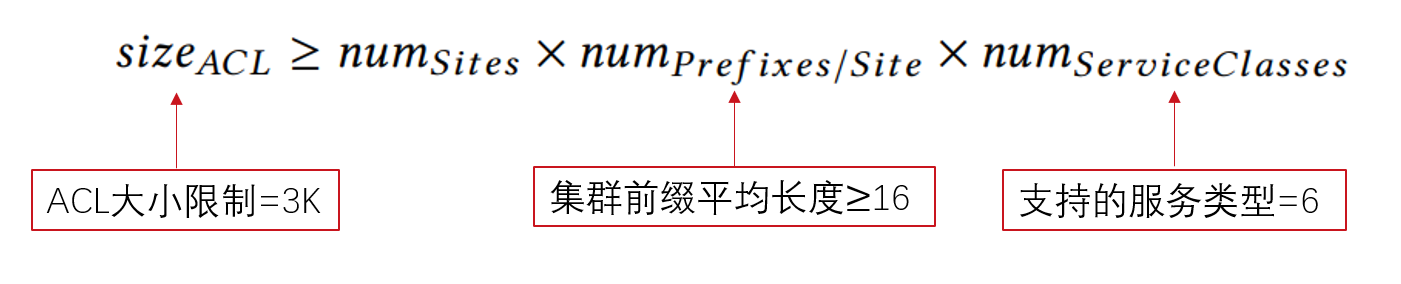
\includegraphics[width=0.7\linewidth]{img/FG.png}
        \label{fig:my_label}
    \end{figure}
    计算后可知,当站点个数达到32左右,将会超过ACL的大小限制。
\end{frame}

\begin{frame}{FG 匹配}
    \framesubtitle{对比}
    基于\highlight[csecondary]{最长前缀匹配}的层级 FG 匹配可以大幅减少匹配流表数量,以增大支持的站点数量。
    \begin{columns}
        \begin{column}{0.4\textwidth}
            \begin{figure}
                \centering
                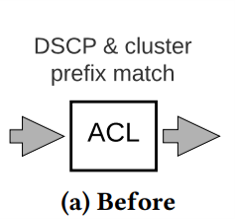
\includegraphics[width=0.4\linewidth]{img/FG2.png}
                \caption{最大支持站点数量:\textbf{32}}
            \end{figure}
        \end{column}
        \begin{column}{0.4\textwidth}
            \begin{figure}
                \centering
                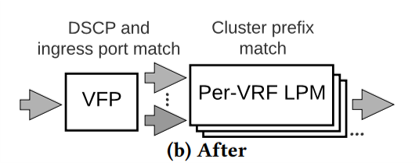
\includegraphics[width=0.8\linewidth]{img/FG3.png}
                \caption{最大支持站点数量:\textbf{1920}}
            \end{figure}
        \end{column}
    \end{columns}
\end{frame}

\begin{frame}{FG 匹配}
    \framesubtitle{层级 FG 匹配}
    %     将FG匹配换分为两个层次化阶段:
    % \begin{enumerate}
    %     \item 将集群前缀匹配迁移至LPM表,LPM表项远多于ACL表。
    %  \item 利用LPM表匹配虚拟路由转发(VRF)标签,通过虚拟转发平面(VFP)表匹配DSCP标记,使得匹配的数据包进入交换机流水线的LPM表之前可以关联一个VRG标签标示其相应的服务等级。
    % \end{enumerate}
    由于 LPM\footnote{Longest Prefix Matching,最长前缀匹配。} 表项远多于ACL表,但是 LPM 表并不能直接与 DSCP 标签匹配却可以与虚拟路由转发(VRF)标签匹配,所以首先采用 虚拟转发平面(VFP)生成VRF。
    \begin{columns}
        \begin{column}{0.6\textwidth}
            \begin{algorithm}[H]
                \caption{层级 FG 匹配}\label{alg:fgmatch}
                将 DSCP 标签先通过 VFP 匹配到一个 VRF 以确定相应的服务等级\;
                结合 VRF 对集群前缀匹配于 LPM表\;
            \end{algorithm}
        \end{column}
        \begin{column}{0.4\textwidth}
            \begin{figure}
                \centering
                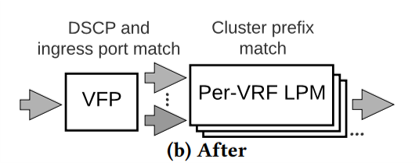
\includegraphics[width=\linewidth]{img/FG3.png}
            \end{figure}
        \end{column}
    \end{columns}

\end{frame}

\begin{frame}{FG 匹配}
    \framesubtitle{其他特性}
    当TE发生某些致命错误时,可以在源站点禁用TE,暂时退回到BGP/ISIS。在入口站点的交换机上删除TE转发规则,数据包可以匹配较低优先级的BGP/ISIS转发规则,而无需封装。
\end{frame}

\begin{frame}{分流}
    \framesubtitle{最初设计}
    最初,仅在入口边缘交换机实现划分TG, TSG, SSG
    % \begin{figure}
    %     \centering
    %     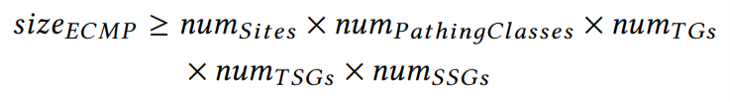
\includegraphics[width = 0.7\linewidth]{img/TS1.png}
    %     \label{fig:my_label}
    % \end{figure}
    \begin{equation*}
        \only<1>{size_{ECMP}}\only<2>{198000}\geq \only<1>{num_{Sites}}\only<2>{33} \times num_{PathingClasses} \times num_{TGs} \times num_{TSGs} \times num_{SSGs}
    \end{equation*}
    \only<1>{
        \begin{enumerate}
            \item $num_{PathingClasses}$是共享共同路径约束的服务类的数量,其值为3
            \item $num_{TGs}$是隧道分割的颗粒度,其值为4
            \item $num_{TSGs}$是每个超级节点的分割粒度,其值为32
            \item $num_{SSGs}$是Stargate后端阶段可供分配的交换机个数,其值为16
        \end{enumerate}
    }
    \only<2>{
        当$num_{sites}$取33时,$size_{ECMP}$至少为198K,但实际上,交换机只支持$size_{ECMP}$不超过14K,可以通过降低数据分流的颗粒度来降低所需的ECMP条目,但是这会填平TE带来的优势,\highlight{需要前后端分离}。
    }
\end{frame}

\begin{frame}{分流}
    \framesubtitle{基于划分的高效流量哈希}
    \begin{columns}
        \begin{column}{0.6\textwidth}
            \begin{algorithm}[H]
                \caption{基于划分的高效流量哈希}\label{alg:hash}
                在一个 CLOS 集群上,边缘交换机决定采用哪个隧道(TG 分流)并判断入端数据流应被发送到哪个站点(TSG分流第\uppercase\expandafter{\romannumeral1}步)。用一特殊的 MAC 标识本地/下一跳结果\;
                后端交换机判断该数据包应被发送到哪个超级节点上(TSG 分流第\uppercase\expandafter{\romannumeral2}步),并判断哪些出边缘交换机与该超级节点有链接(SSG分流)\;
            \end{algorithm}
            并对可用的后端交换机添加 LAG(Link Aggregation Group)以进一步减少入口边缘交换机分配规则。
        \end{column}
        \begin{column}{0.4\textwidth}
            \begin{figure}
                \centering
                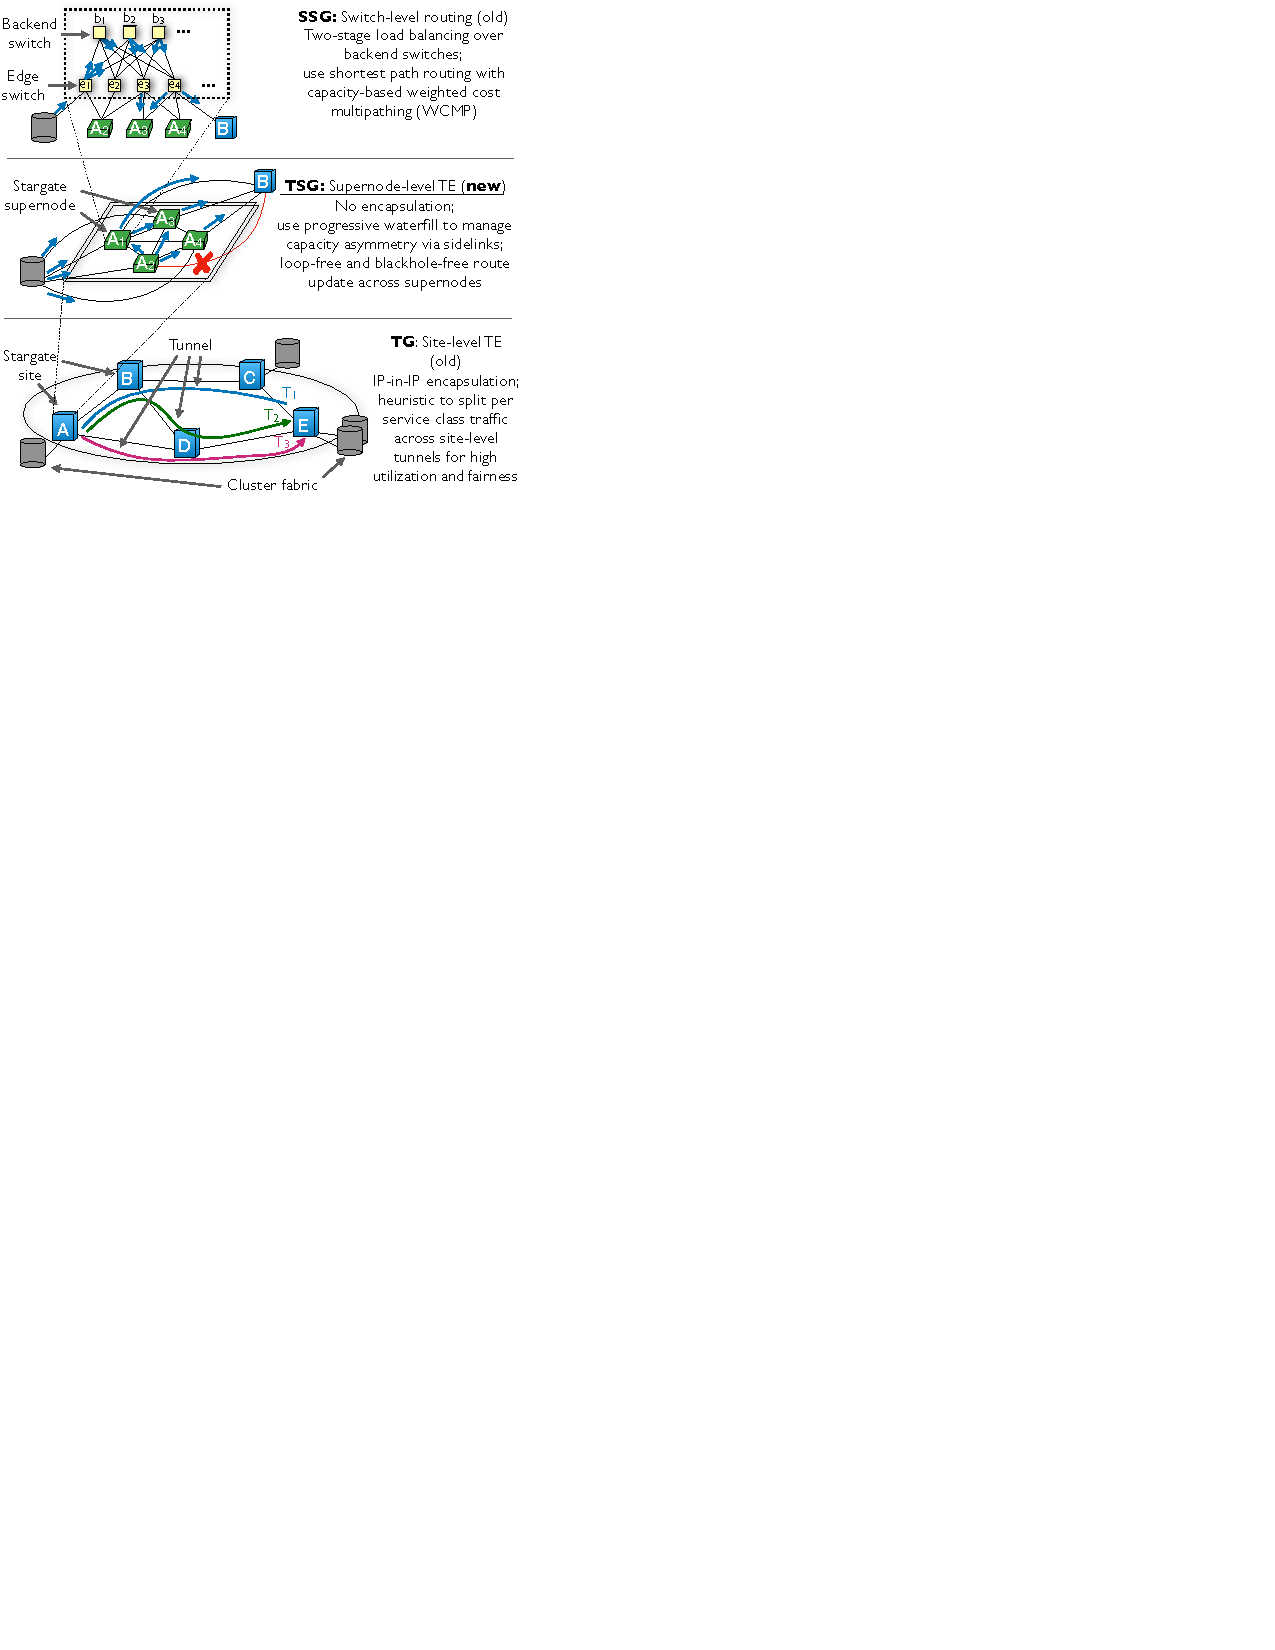
\includegraphics[width=\linewidth,trim={0 6cm 0 0},clip]{hitearch}
            \end{figure}
            \begin{table}
                \centering
                \caption{分流判断负载对比}
                \begin{tabular}{c|p{2cm}|p{1.5cm}}
                    \toprule
                         & \bfseries Before & \bfseries After                                  \\
                    \hline
                    边缘 & TG, TSG, SSG     & TG, TSG(\uppercase\expandafter{\romannumeral1})  \\
                    \hline
                    后端 &                  & TSG(\uppercase\expandafter{\romannumeral2}), SSG \\
                    \bottomrule
                \end{tabular}
            \end{table}
        \end{column}
    \end{columns}
\end{frame}

\section{评估}
%\subsection{规模}
\begin{frame}
    \frametitle{规模}
    \framesubtitle{总流量}
    \begin{columns}
        \begin{column}{0.4\textwidth}
            \begin{figure}
                \centering
                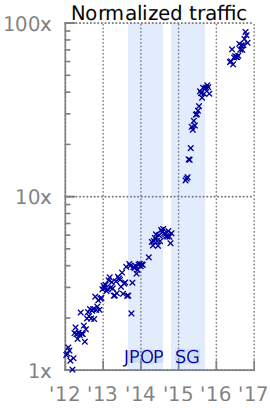
\includegraphics[height=0.6\textheight]{1_a.png}
                \caption{归一化到最小值的流量总量}
            \end{figure}
        \end{column}

        \begin{column}{0.6\textwidth}
            \begin{itemize}
                \item 五年内,总流量增长了两个数量级;平均每9个月,流量就增加一倍
                \item 相较于面向互联网的广域网,B4提供了更多的流量,并且增长速度更快
            \end{itemize}
        \end{column}
    \end{columns}
\end{frame}

\begin{frame}
    \frametitle{规模}
    \framesubtitle{站点与控制域的数量}
    \begin{columns}
        \begin{column}{0.4\textwidth}
            \begin{figure}
                \centering
                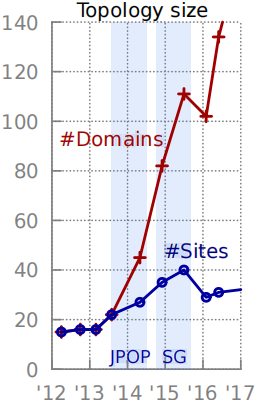
\includegraphics[height=0.6\textheight]{1_b.png}
                \caption{站点和控制域的数量}
            \end{figure}
        \end{column}

        \begin{column}{0.6\textwidth}
            \begin{itemize}
                \item 基于Saturn时,二者数量一致;从2013年部署JPOP以后出现分歧
                \item 2015年,为了提高可拓展性,大大减少了Saturn的站点数量,将其替换为Stargate。但由于在迁移期间,Saturn和Stargate会暂时在一个站点内共存,这反而带来了可拓展性问题。
            \end{itemize}
        \end{column}
    \end{columns}
\end{frame}

\begin{frame}
    \frametitle{规模}
    \framesubtitle{Flow Group}
    \begin{columns}
        \begin{column}{0.4\textwidth}
            \begin{figure}
                \centering
                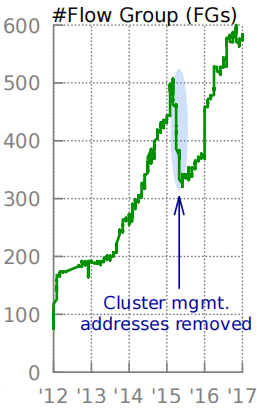
\includegraphics[height=0.6\textheight]{1_c.png}
                \caption{每个站点的FG数}
            \end{figure}
        \end{column}

        \begin{column}{0.6\textwidth}
            \begin{itemize}
                \item 过去的五年中,平均每个源站点的Flow Group增加了六倍
                \item 2015年,停止向交换机和supertrunk端口分发IP地址,这使Flow Group减少了约30\%
            \end{itemize}
        \end{column}
    \end{columns}
\end{frame}

\begin{frame}
    \frametitle{规模}
    \framesubtitle{Tunnel Group}
    \begin{columns}
        \begin{column}{0.4\textwidth}
            \begin{figure}
                \centering
                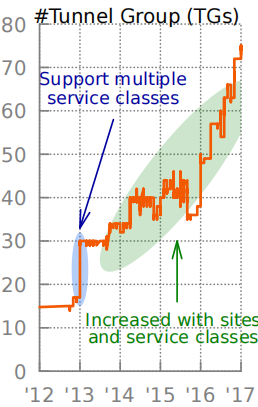
\includegraphics[height=0.6\textheight]{1_d.png}
                \caption{每个站点的TG数}
            \end{figure}
        \end{column}

        \begin{column}{0.6\textwidth}
            \begin{itemize}
                \item 2013年初,开始支持多个服务级别,这使得每个站点的TG数翻了一番
                \item 此后,随着站点数和服务级别的增加,每个站点的TG数持续增长
            \end{itemize}
        \end{column}
    \end{columns}
\end{frame}

\begin{frame}
    \frametitle{规模}
    \framesubtitle{隧道数}
    \begin{columns}
        \begin{column}{0.4\textwidth}
            \begin{figure}
                \centering
                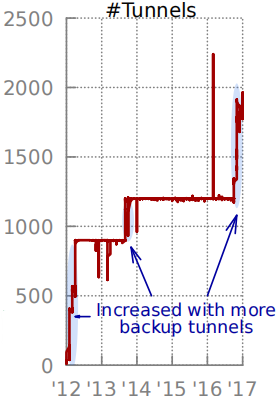
\includegraphics[height=0.6\textheight]{1_e.png}
                \caption{每个站点的传输隧道数}
            \end{figure}
        \end{column}

        \begin{column}{0.6\textwidth}
            \begin{itemize}
                \item 每个站点的传输隧道数由中央控制器的配置调控,这有助于避免配置过多的交换规则,但也限制了备份隧道的数量
                \item 2016年,随着交换规则管理的改进,提高了可安装备份隧道的数量
            \end{itemize}
        \end{column}
    \end{columns}
\end{frame}

\begin{frame}{可用性}
    \paragraph{基于带宽的有效性}
    \begin{equation*}
        \frac{allocation}{min\{demand, approval\}}
    \end{equation*}
    其中,demand是基于短期内的历史使用情况评估的,approval是每个SLO所允许的最小带宽,allocation指当前带宽,它受到网络容量和公平性的约束。
    \paragraph{基于连通性的有效性}对于每一个服务级别,通过一个网络测量系统对每个集群对进行测量。每一个集群对的有效性定义如下:
    \begin{equation*}
        \begin{cases}
            1,                                    & loss\_rate\leq\alpha \\
            10^{-\beta\times(loss\_rate-\alpha)}, & otherwise
        \end{cases}
    \end{equation*}
    其中,$\alpha=5\%$是一个灵敏度阈值,它过滤掉了大部分的瞬态损失,同时捕获了会影响有效性的更大的损失。超过阈值后,随着传输损失率的提高,有效性成指数级下降,衰减因子$\beta=2\%$。
\end{frame}

\begin{frame}
    \frametitle{可用性测量结果}
    \begin{figure}
        \centering
        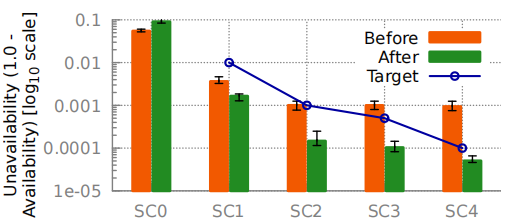
\includegraphics[height=0.5\textheight]{6.2.png}
        \caption{每个服务级别的测量到的和目标需要的不可用性} %
    \end{figure}

    \begin{itemize}
        \item 取上述两个指标的最小值作为网络有效性
        \item 对于每一个服务类,B4都达到了目标有效性
    \end{itemize}
\end{frame}

%\subsection{Design Tradeoffs}

\begin{frame}
    \frametitle{设计折衷}
    \framesubtitle{拓扑抽象化}
    %\framesubtitle{Topology abstraction}   
    为了更少的容量损失进行拓扑抽象。
    \begin{figure}[h]%%图
        \centering  %插入的图片居中表示
        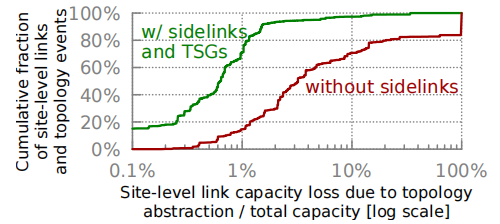
\includegraphics[height=0.5\textheight]{fig11.png}
        \caption{由分层拓扑中的容量不对等造成的容量损失}  %图片的名称
    \end{figure}
\end{frame}

\begin{frame}
    \frametitle{设计折衷}
    \framesubtitle{带有两级哈希的分层结构TE}
    \begin{columns}
        \begin{column}{0.4\textwidth}
            \begin{figure}[h]%%图
                \centering  %插入的图片居中表示
                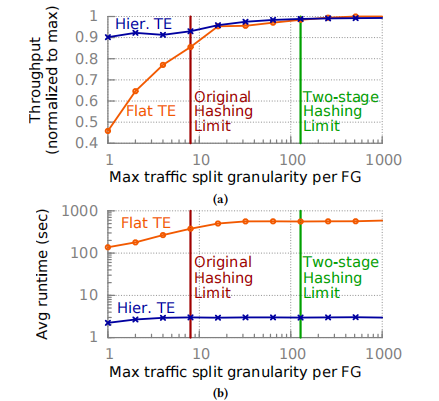
\includegraphics[width=\linewidth]{fig12.png}
                \caption{吞吐量和平均运行时间比较}  %图片的名称
            \end{figure}
        \end{column}
        \begin{column}{0.6\textwidth}
            \begin{itemize}
                \item 分层结构TE的运行时间仅为2-3秒,比扁平结构TE快188倍。
                \item 当最大流量分割间隔设置为1时,不论是分层结构还是扁平结构性能都很差,其吞吐量分别少于对应结构最大吞吐量的91\%和46\%。
                \item 在最初的8路分流中,分层结构TE只实现了其最大吞吐量的94\%。
            \end{itemize}
        \end{column}
    \end{columns}
\end{frame}

\begin{frame}
    \frametitle{设计折衷}
    \framesubtitle{TSG排序}
    \begin{columns}
        \begin{column}{0.4\textwidth}
            \begin{figure}
                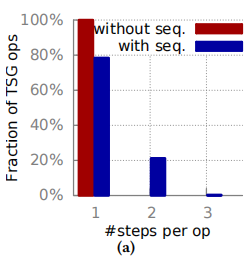
\includegraphics[height=0.7\textheight]{fig13a.png}
                %\caption{}
            \end{figure}
        \end{column}
        \begin{column}{0.6\textwidth}
            \begin{itemize}
                \item 在超过99.7\%的TSG操作中,TSG排序只需要一或两个“步骤”。
                \item 每个步骤由一个或多个TSG更新组成,其中它们的相对顺序不被强制执行。
            \end{itemize}
        \end{column}
    \end{columns}
\end{frame}

\begin{frame}
    \frametitle{设计折衷}
    \framesubtitle{TSG排序}
    \begin{columns}
        \begin{column}{0.4\textwidth}
            \begin{figure}
                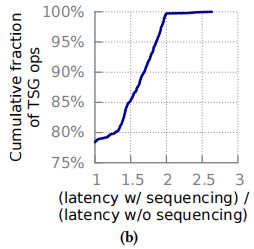
\includegraphics[height=0.7\textheight]{fig13b.png}
                %\caption{}
            \end{figure}
        \end{column}
        \begin{column}{0.6\textwidth}
            \begin{itemize}
                \item 在99.7百分位时,延迟增加了2倍,最坏情况下增加2.63倍。
                \item TSG排序算法的运行时相对于编程延迟可以忽略不计。
            \end{itemize}
        \end{column}
    \end{columns}
\end{frame}

\begin{frame}
    \frametitle{设计折衷}
    \framesubtitle{TSG排序}
    \begin{columns}
        \begin{column}{0.4\textwidth}
            \begin{figure}
                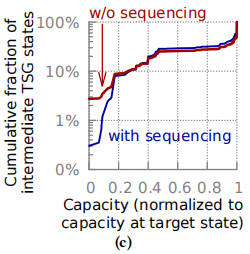
\includegraphics[height=0.7\textheight]{fig13c.png}
                %\caption{}
            \end{figure}
        \end{column}
        \begin{column}{0.6\textwidth}
            \begin{itemize}
                \item 没有排序:可用容量因出现黑洞/循环降至零的可能性约为在3\%。
                \item 有排序:这个可能性将被降低一个数量级。
            \end{itemize}
        \end{column}
    \end{columns}
\end{frame}

\begin{frame}
    \frametitle{设计折衷}
    \framesubtitle{TSG排序}
    \begin{columns}
        \begin{column}{0.4\textwidth}
            \begin{figure}
                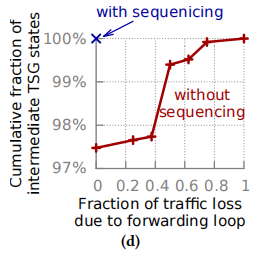
\includegraphics[height=0.7\textheight]{fig13d.png}
                %\caption{}
            \end{figure}
        \end{column}
        \begin{column}{0.6\textwidth}
            \begin{itemize}
                \item 在没有排序的情况下,TSG运行时,有超过2\%的中间状态中形成转发循环,这导致超过 超过38\%的入口流量将被丢弃。
            \end{itemize}
        \end{column}
    \end{columns}
\end{frame}

\section{运营经验和待解决问题}
\begin{frame}{简化管理}
    \begin{enumerate}
        \item 升级前,需要手动计算由于容量不对称而造成的容量损失,以保证降级的站点容量仍然满足流量需求;升级后,需要人工干预之处大大减少,因为TE系统能够自动且高效的处理不对称容量。
        \item 限制操作范围至一次一个域,以减小潜在的影响;使用影响分析工具对网络情况进行监控,通过结果判断某些请求是否被接受。
        \item 由于B4网络的大规模,由命令行控制网络“排水”操作是不现实的,这一操作由管理工具调用,这些工具通过管理RPC来协调网络操作。
    \end{enumerate}

\end{frame}

\begin{frame}
    \paragraph{确定旁路容量} 确定应部署的最佳旁路容量以满足带宽保证是一个非常困难的问题,Google正在研究一个日志驱动的统计分析框架以解决该问题。

    \paragraph{处理不平衡输入流量} TSG算法默认入端流量是平衡的,优势在于,管道可以共享TSG规则,而不用对每个管道都去分配一套规则(这样做会超过硬件规则极限),但缺点在于,对不平衡的流量处理能力较差。Google尝试开发计算每对相邻站点级链接的TSG规则的算法进行优化。
\end{frame}

\begin{frame}{相关工作}
    \begin{itemize}[<+->]
        \item \highlight[csecondary]{Software-defined WAN}  一些公司也已经将SDN用于数据中心间的连接,如Facebook、微软SWAN等。Google认为他们发展B4的经验也可以应用于这些工作。

        \item \highlight[csecondary]{Decentralized, hierarchical network abstractions} 分层路由的概念由来已久,近年来也有不少去中心化的、分层式的SDN路由架构被提出。B4是以这些概念为基础构建出来的,Google认为其创新点在于克服了将这些众所周知的概念应用于全球规模时所面临的实际挑战。

        \item \highlight[csecondary]{TE and WAN resource scheduling} 诸如Tempus, Pretium, SOL, FFC 等创新性的概念是可以被运用到B4中以优化其控制和数据层面的。

        \item \highlight[csecondary]{Network update and switch rule management} B4中的TSG 排序不需要数据包标注即可解决限制性网络使用案例,这与同领域其他工作是不同的;解耦转发规则这一概念在很多过往的工作中已被应用,B4中,这一方案的独特之处在于,揭示了当规模足够大时,扩大交换机规则管理方面面临的挑战。
    \end{itemize}

\end{frame}

\section{总结}
\begin{frame}{总结}
    该论文介绍了本文介绍了Google团队将B4从一个以\alert{99\%}的可用性为目标的批量传输、内容复制网络发展到支持需要\alert{99.99\%}可用性的交互式网络服务的网络的历程和经验。主要是通过将B4重新架构为分层拓扑结构,同时开发TE算法和交换机规则管理机制来进行升级。高可用性、带宽充足的网络对众多云服务有着重要贡献,Google团队也正努力继续优化B4网络,使其可用性再次得到提高。
\end{frame}

\begin{frame}[plain]
    \frametitle{分工}
    \begin{itemize}
        \item 李子龙:演讲、第 6 节
        \item 张 露:第 1、2 节
        \item 李婉婷:第 3、4 节
        \item 田淏元:第 5、7 节
    \end{itemize}
\end{frame}

\makebottom[min]
\end{document}